
% to choose your degree
% please un-comment just one of the following
\documentclass[bsc,frontabs,twoside,singlespacing,parskip,deptreport]{infthesis}     % for BSc, BEng etc.
% \documentclass[minf,frontabs,twoside,singlespacing,parskip,deptreport]{infthesis}  % for MInf

\usepackage{amsmath}

% \usepackage[bitstream-charter]{mathdesign}
\usepackage{fixltx2e}
\usepackage[english]{babel}
\usepackage{microtype} % removes extra spacing between text
\usepackage{ragged2e}
%\usepackage{lscape} % to write pages in landscape environment
\usepackage{array, threeparttable} % to add footnotes to the tables
% \usepackage{caption} % to create some space between table caption and table, otherwise there was no space
% \captionsetup[table]{skip=5pt}
% \usepackage[singlelinecheck=false]{caption}

\usepackage{graphicx}
\usepackage[absolute,overlay]{textpos}
\usepackage{eushield}
\shieldtype{3}
\usepackage{graphicx}
\usepackage{float}
\usepackage{lipsum}
\usepackage{enumitem}
\usepackage{booktabs}
\usepackage{tabularx}
\usepackage{mathtools,amssymb}
\usepackage{enumitem}
\usepackage{todonotes}
\usepackage{amsmath}
\usepackage[utf8]{inputenc}
\usepackage{amssymb}
\usepackage{hyperref}
\usepackage{gensymb}
\usepackage{longtable}
\usepackage[titletoc]{appendix}
\usepackage{blindtext}
\usepackage{lscape}
\usepackage{csvsimple}
\usepackage{graphicx}
\usepackage{subcaption}
\usepackage{algorithm,algpseudocode}
\usepackage{amsmath}
\usepackage{amsfonts}
\usepackage{amssymb}
\renewcommand{\algorithmicrequire}{\textbf{Input:}}
\renewcommand{\algorithmicensure}{\textbf{Output:}}

\usepackage{hyperref,xcolor}% http://ctan.org/pkg/{hyperref,xcolor}
\usepackage{makeidx}
\definecolor{winered}{rgb}{0.5,0,0}
\usepackage{xcolor}


\hypersetup{
  colorlinks   = true, %Colours links instead of ugly boxes
  urlcolor     = black, %Colour for external hyperlinks
  linkcolor    = blue, %Colour of internal links
  citecolor   = winered %Colour of citations
}

\usepackage{graphicx}
\usepackage[absolute,overlay]{textpos}
\usepackage{eushield}
\shieldtype{3}
\begin{document}
% \begin{textblock*}{<hsize>}(<hpos>,<vpos>)
\begin{textblock*}{100pt}(16cm,2cm)
\includegraphics[width=80pt]{\eushield}
\end{textblock*}

\title{Predicting Corporate Bankruptcy using Ensemble Learning}

\author{Ishan Rohan Parikh}

% to choose your course
% please un-comment just one of the following
\course{Artificial Intelligence and Computer Science}

% to choose your report type
% please un-comment just one of the following
\project{Undergraduate Dissertation} % CS&E, E&SE, AI&L
%\project{Undergraduate Thesis} % AI%Psy
\project{4th Year Project Report}

\date{\today}

\abstract{
Bankruptcy prediction has been a subject of interest for almost a century and leading to intensive research from academics and practitioners. The aim of predicting financial distress is to develop a predictive model that combines various econometric measures and allows us to foresee the financial condition of a firm. Seminal academic research has evaluated bankruptcy prediction using traditional statistics techniques (e.g. Logistic Regression) and early artificial intelligence models (e.g. Artificial Neural Networks).

In this study, we use ensemble machine learning models to predict bankruptcy on a one-year horizon. 
We use Wharton Research Data Services to provide financial data from 4000 listed Japanese corporations.
Using financial data from 2000 to 2018, our study uses 64 financial ratios chosen from the seminal research, as documented in \cite{Altman,beaver2005have,hardle2009variable,tian2017financial,tian2015variable, ding2012class}.
This research leads to a substantial improvement in prediction performance using different imputation techniques to estimate missing data and the creation of synthetic minority class data using the Synthetic Minority Over-sampling Technique (SMOTE). We compare the performance of machine learning and ensemble learning techniques, specifically Decision Trees, Random Forests, Bagging, and Extreme Gradient Boosting (XGBoost). 

We find that using Multiple Imputation by Chained Equations as an imputation technique and XGBoost as an ensemble model, outperforms the other models by achieving the highest AUC and F1 score of 0.856 and 0.798 respectively. 
Our research adds to the discussion and the ongoing debates about the superiority of computational methods over statistical techniques, as seen in Tsai, Hsu, and Yen's \cite{tsai2014comparative} and Yeh, Chi, and Lin's papers \cite{yeh2014going}. We also put forward a novel contribution towards Japanese bankruptcy prediction by using a ten-year rolling window model on our data and then pipelining it into an ensemble prediction framework.
}

\maketitle

\section*{Acknowledgements}
I would like to take this opportunity to thank my supervisor, Dr. Tiejun Ma, for providing me with the necessary financial data for this project and for guiding me through the course of this dissertation. Dr. Ma encouraged me to do a very thorough study of the existing research, which helped me in exploring newer ideas. 

I also want to acknowledge the contribution of Mr. Luo Chang, for his limitless patience and mentorship during my project. His advice on how to do effective research saved me countless hours, which was then invested in documenting this project.

My dissertation submission is amidst a worldwide COVID-19 pandemic being suffered by millions across the world. At the time of a nationwide lockdown, away from University, I am eternally grateful to my friend Liam and his parents Mair and Peter for extending their home and heart to me.

Finally, to my family, for giving me this opportunity to study at the University of Edinburgh and for their constant support and encouragement to pursue all the opportunities in front of me and always inspiring me to do my best by going beyond the defined lines to raise the bar.

\tableofcontents

%\pagenumbering{arabic}


\chapter{Introduction}
Predicting corporate bankruptcy is important because business failures have wide ranging repercussions. It affects internal and external stakeholders of the company such as management, employees, shareholders, creditors, suppliers, clients, governments and global economies \cite{shumway2001forecasting}. Corporate bankruptcy can destabilise the economic system by increasing the unemployment rate, depriving investors and creditors of livelihood and contributing to a higher the crime rate  \cite{mbat2013corporate}. On a large scale, it can lead to negative micro and macro‐economic consequences affecting multiple stakeholders and potentially cause social dislocation, economic downturns and recessions \cite{jones2008advances}.

% Although default events behave stochastically, capital market information can be used to develop bankruptcy prediction models. 
Beaver \cite{beaver1967financial} and Altman \cite{Altman} were pioneers in predicting bankruptcies and their work is still referenced and valid today. As there are no mature theories of corporate bankruptcy, most studies in corporate bankruptcy are largely been based on iterative, trial and error processes that involve selecting features (such as $\frac{Working \mbox{ }Capital}{Total \mbox{ } Capital}$, $\frac{Retained  \mbox{ }Earnings}{Total \mbox{ } Assets}$, etc.) and predictive models \cite{zhou2014bankruptcy}. 

Early statistical methods applied in corporate bankruptcy prediction utilised Linear Discriminant Analysis (LDA) and Logistic Regression Analysis (LRA) \cite{li2009gaussian}. The problem with applying these statistical techniques to bankruptcy prediction is that the assumptions for independent variables are frequently violated in the practice, which makes these techniques theoretically invalid for finite samples \cite{shin2002genetic}. 

To overcome these limitations, intelligent techniques that do not assume certain data distributions and automatically extract knowledge from training samples have been developed actively in the field of machine learning \cite{alaka2018systematic,lessmann2015benchmarking}. Machine learning models like Support Vector Machines (SVMs), Neural Networks (NNs) and ensemble models have been reported to be more accurate than the traditional statistical methods as shown in \cite{barboza2017machine}. 

% However, there still isn't an conclusive technique devised to effectively predict corporate bankruptcies. 
% The devil is in the details when it comes to prediction accuracy. These include the data structure, the features or financial ratios used, the extent to which it is possible to segregate the classes, the objective of the classification, etc \cite{duenez2013no}. 
Although numerous previous studies concluded that machine learning techniques are superior to statistical models, it has been argued that no 'single' classifier can produce the best results. Results also tend to vary when models are tested on data from different countries and economies.

Recently, integrating multiple predictors into an aggregated output, i.e., ensemble methods, have been demonstrated to be an efficient strategy in predicting bankruptcies, especially when the component predictors have different structures that lead to unique prediction errors \cite{breiman1996bagging}. Moreover, latest studies have shown that such ensemble techniques are better performers than single intelligent techniques in financial distress prediction \cite{deligianni2012forecasting,sun2012financial}.


With the discovery of Extreme Gradient Boosting (XGBoost) in 2016, ensemble learning has made major advances in solving real world data driven problems that have resisted the determined attempts of the artificial intelligence community for many years.
It has turned out to be very successful at discovering intricate structures in high-dimensional data and is, therefore applicable to many domains of science, business and government. In addition, ensemble learning has been predicted to have many more successes in the near future, largely because they require very little engineering by hand and can be run very efficiently and achieve credible performance \cite{chen2020ensemble}. 
% Consequently, ensemble learning can take advantage of large datasets with an increased computational ca
% increase in the amount of available  ability and data. 

Financial ratios are relationships determined from a company's financial information and is used for comparison purposes. Some examples include measures such as return on investment (ROI), return on assets (ROA), and debt-to-equity, etc. These ratios are the result of dividing one account balance or financial measurement with another. 
% Usually these measurements or account balances are found on one of the company's financial statements—balance sheet, income statement, cashflow statement, etc.
They describe the financial health of companies and measure different aspects of a company's performance. Since these ratios are often characterised by high variance, they often tend to pose as a problem for machine learning algorithms.
This problem is also difficult to overcome when data is normalised or standardised. 
Ensemble methods that use tree-based learners take into account the order of feature values, not the values itself. Therefore, they are resistant to the large variance observed in the economic indicators. 

Ensemble models are among the most effective methods for improving recognition of the minority class, this makes ensembles robust to class imbalance and reduces overfitting. They can also employ preprocessing methods before learning component classifiers or embed a cost-sensitive framework in the ensemble learning process \cite{blaszczynski2017actively}.


\section{Motivation and Goals}
For financial institutions, the ability to accurately predict in advance any possible business failures is crucial, as incorrect decisions can have direct and severe economical consequences. Our objective is to help address this problem by building a highly effective bankruptcy prediction model and test its performance on financial data from listed Japanese companies. We propose the use of ensemble learning to build these bankruptcy prediction models as ensembles have emerged as a powerful tool that leverage a pool of individual (base) learners and produce highly accurate classification models.
Practical investigations have demonstrated that ensembles with tree-based base learners generally outperform stand-alone prediction methods in most credit risk and bankruptcy prediction problems \cite{west2005neural,doumpos2007model,alfaro2008bankruptcy,sun2012financial}. 
Research has also shown that using ensemble models to predict bankruptcy has been able to outperform complex models like neural networks \cite{kim2010ensemble}. 
% is to conduct an in-depth analysis to understand the numerous characteristics and complexities of financial data. 
% Gaining an understanding of this, we take the approach of designing machine learning models with the help of ensembles to accurately predict corporate bankruptcy.
% we explore the potential links between the performance of classifier models and provide a detailed evaluation of them.
% ensembles are emerg- ing as a powerful tool for exploiting the different behaviour of a pool of individual learners and also in reducing prediction errors in several financial applications, we take the approach of leveraging these models to accurately predict corporate bankruptcy


% for exploiting the different behaviour of a pool of individual learners 



% We aim to contribute this field of literature by putting forth a novel contr

% showing that powerful ensemble methods were used to make bankruptcy predictions Japanese companies.

% To the best of our knowledge, our study puts forth a novel contribution on the Japanese dataset, wherein we consider the financial condition of listed Japanese companies from 2000 to 2018. We compare the results obtained on the bankruptcy prediction task using different machine learning and ensemble models.


\section{Work Completed and Personal Contributions}

% This paper carries out a meticulous data analysis on the financial health of listed Japanese companies from 2000 to 2018.To the best of our knowledge our paper puts forth a novel approach of predicting bankruptcy by demonstrating it through Japanese financial data. Based on the success seen in \cite{matsunaga2019exploring,li2019dp,molodtsova2009out}, we employ a ten year rolling window for five consecutive years and predict bankruptcy - using imputation techniques, oversampling and ensemble learning - in a one year horizon.

To the best of our knowledge this paper puts forth a novel contribution to the bankruptcy prediction problem by using a ten year rolling window model to predict bankruptcy on a one year horizon. The Asian economy is often ignored in financial research - the paucity of available resources is representative of this. As Japan has the third highest market capitalisation in the world, we chose to carry out our research on the Japanese economy.
After conducting a meticulous data analysis on the financial health of listed Japanese companies from 2000 to 2018, we compare three imputation techniques along with oversampling the minority class and then use ensemble learning to produce results that are in line with similar research on different economies \cite{barboza2017machine,le2018cluster}.

We aim to address the gap in literature by comparing the performance of different data imputation\footnote{Imputed value is an assumed value given to an item when the actual value is not known or available. Imputed values are a logical or implicit value for an item or time set, wherein a "true" value has yet to be ascertained. It would be a best guess estimate, to accurately estimate a larger set of values or series of data points.} techniques that could be used to estimate missing data. Additionally, efforts have been made to account for the class imbalance by including a stage of over sampling of the minority class.
Machine Learning models have been implemented and their results have been critiqued and compared to produce the best prediction model for the available dataset. A case has been made for the ability of ensemble models to prevent overfitting by achieving high F1-Scores and AUC values under the ROC curve.


Henceforth the paper is organised as follows: In \autoref{chap:LiteratureReview}, we conduct a background review of related financial and machine learning research. In \autoref{chap:JapanDataset}, we describe and the Japanese financial dataset, its relevance in being representative of the modern markets and also summarise some key statistics and features that provide a general overview on the data. We also discuss the data pre-processing steps that have been used.
In \autoref{chap:Methodologies}, we outline our experiment methodologies and describe the evaluation metrics that have been used. In \autoref{chap:Results}, we present our empirical results. In \autoref{chap:Discussion} we discuss the results obtained in the light of existing literature and put forward our best performing model. We conclude in \autoref{chap:Conclusion} with a summary of the main findings, the implications of this work and suggested areas for further research.



%% --------------------------       NEW CHAPTER BEGINS HERE         ------------------------------
\chapter{Background and Literature Review}
\label{chap:LiteratureReview}

At the time of writing in 2020, with a  US recession\footnote{This study has not been updated to account for the market crash due to the COVID-19 pandemic.} on the horizon (as shown by data produced by Bloomberg in \autoref{fig:US_recession_prob}), the need for risk assessment is increasingly important to avoid repeating the carnage caused by the 2008 financial crisis. 
While in the past the small and medium (and micro) companies had higher propensity of going bankrupt, more recently we have also seen an uptick in bankruptcies of large global firms. A few examples are the big retail companies such as Toys``R"Us, Debenhams, Forever 21, JC Penney and Sears. The travel agency Thomas Cook and the low-cost airline Flybe have also filed for bankruptcy in the past two years.

% \begin{figure}[htp]
% \centering
% % \captionsetup{justification=centering}
  
%   \centering
%     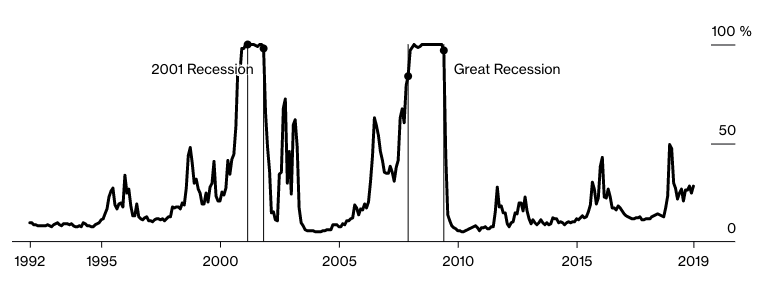
\includegraphics[height=5cm,width=\columnwidth]{Images/recessionUs.png}
%   \caption{Probability of U.S. recession within 12 months. \\
%   Source: \href{https://www.bloomberg.com/graphics/us-economic-recession-tracker/}{Bloomberg}}
%  \label{fig:US_recession}
% \end{figure}
The global recession in 2008 proved that companies were inappropriately evaluated by credit rating agencies and banks. Governments around the world were forced to implement trillion-dollar rescue packages to keep the plumbing behind banking systems running. Given the devastating effects of the financial crisis on firms, now, more than ever, there is a need to identify (and anticipate) upcoming bankruptcies. The surge in the number of research papers around bankruptcy is increasingly evident from \autoref{fig:numberofcases}. 
% During the decade of 2008-2017, the number of publications has increased significantly, representing 83.50\% of total papers analysed. 
% Boosting the accuracy of credit risk and corporate default methodologies used by banks and financial institutions may lead to considerable gains and have a critical impact on global economies. 

% \begin{figure}[htp]
% \centering
% \captionsetup{justification=centering}
  
%   \centering
%     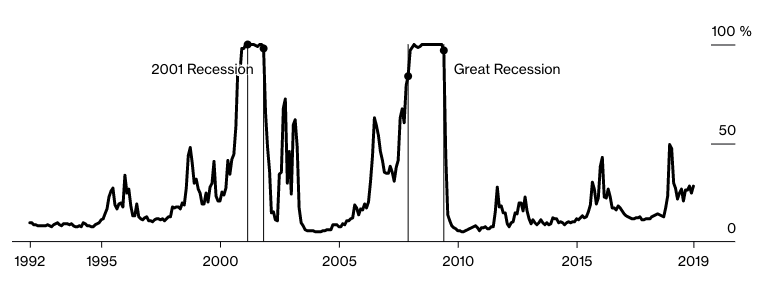
\includegraphics[height=5cm,width=\columnwidth]{Images/recessionUs.png}
%   \caption{Probability of U.S. recession within 12 months. \\
%   Source: \href{https://www.bloomberg.com/graphics/us-economic-recession-tracker/}{Bloomberg}}
%  \label{fig:US_recession}
% \end{figure}

\begin{figure}[htp]
  \centering
%   \captionsetup{justification=centering}
    
      {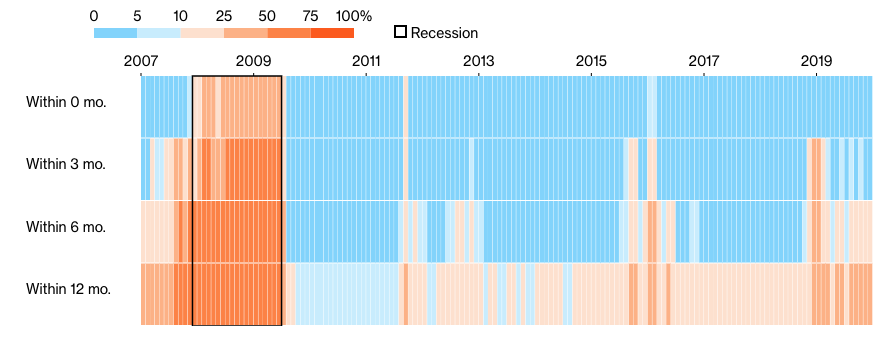
\includegraphics[height=5cm,width=\columnwidth]{Images/recession.png}}
  \caption{Probability of recession within 0, 3, 6 and 12 months \\ 
  Source:\href{https://www.bloomberg.com/graphics/us-economic-recession-tracker/}{Bloomberg}}
  \label{fig:US_recession_prob}
\end{figure}

Situations may arise where a company can become distressed and continue to operate in that condition for many years and can even (at times) recover from their distress. On the other hand, some companies enter bankruptcy immediately after a highly distressing event such as a financial fraud or accounting issues. Several factors influence these outcomes. Lensberg's paper \cite{lensberg2006bankruptcy} investigates related work and categorises numerous factors affecting bankruptcy. Broadly speaking they are audit, financial ratios and fraud indicators, which are measured by qualitative or quantitative variables.
Bankruptcy occurs if a company cannot operate in circumstances, including force majeure events or due to government regulations, or due to its inability to pay off its debt and earn profits for an extended time. 

\begin{figure}[htp]
\centering
% \captionsetup{justification=centering}
  
  \centering
    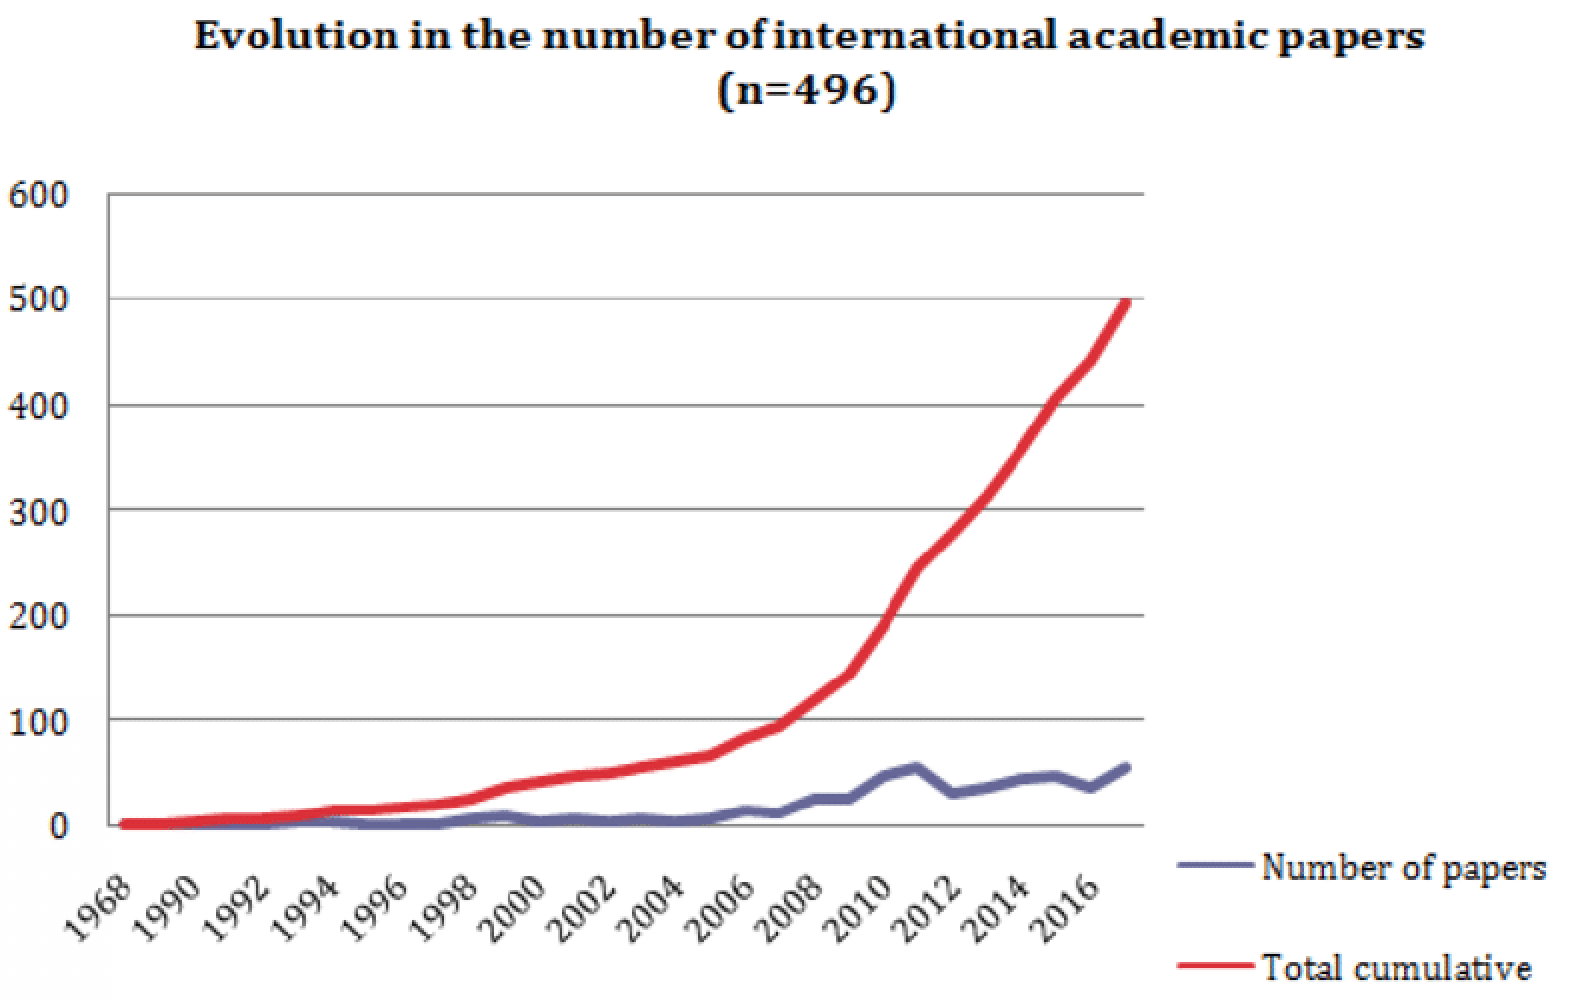
\includegraphics[width=\columnwidth]{Images/evo.png}
  \caption{Rise in the number of international academic articles during the years 1968-2017. This graph has been taken from Shi and Xiaoni's work, published in 2019 \cite{shi2019overview}.}
 \label{fig:numberofcases}
\end{figure}

% Forecasting bankruptcy can be thought of as a classification problem with input variables as the financial, accounting and market data of a firm. Bankruptcy prediction can be stated as a classification problem in the following manner: given a set of parameters (mainly of financial nature) that describe the performance of a company over a given period, what is the probability that the company may become bankrupt during the following year \cite{crone2006impact}.
% Below are some of the reasons for delisting, which can be viewed as de facto bankruptcy: 
% \begin{enumerate}

%     \item Self declaration of bankruptcy/ rehabilitation/ reorganization procedures, 
%     \item Excessive debt
%     \item Suspension of bank transactions, and 
%     \item Termination of business activities (excluding mergers). 
% \end{enumerate}

% In bankruptcy detection, knowing the probability of possible corporate failure is of major importance to all stakeholders since it can help to prevent the adverse effects that such an event can provoke. It is also a key topic related to a measurement of corporate solvency. 
Initial models used in bankruptcy prediction were mainly statistical, such as Multiple Discriminant Analysis \cite{Altman} or Logistic Analysis \cite{ohlson1980financial}. Although these models have been widely used in academia and industry, statistical models are constrained in their ability to increase predictive power. \cite{begley1996bankruptcy}. 
Many recent studies suggest the use of intelligent data mining techniques, including neural networks (NNs), decision trees(DT), case-based reasoning (CBR), support vector machines (SVM), and soft computing \cite{kumar2007bankruptcy}. Neural Networks have an excellent ability to treat non-linear data making them one of the most actively used models in bankruptcy prediction \cite{chandra2010support,baek2003bankruptcy,charalambous2000application}. 

Recent efforts have shown that the performance of predictive models can be significantly enhanced through hybrid and ensemble computing \cite{verikas2010hybrid}. A hybrid system exploits several approaches (e.g., heuristic techniques and classification algorithms) aiming for optimizing the prediction performance. Following this direction, evolutionary algorithms such as genetic algorithm (GA), annealing simulation (AS), particle swarm optimization (PSO), ant colony optimization (ACO), tabu search (TS) are extensively employed in conjunction with machine learning methods \cite{lin2009applying}. The typical usages include tuning the architecture of a particular model (such as the connected weights of MLP \cite{huang2008novel} and the parameters of SVM \cite{min2011tuning}), selecting relevant features, and refining the samples for learning. From another viewpoint, the ensemble approach combines several models and aggregates the output in some rules. It has been shown that a well designed ensemble-based system can outperform a single predictor by inheriting advantages of its base learners.

% \section{Bankruptcy Prediction Models}
% Altman (1968) \cite{Altman} first attempted to simultaneously handle multiple financial ratios. This study used financial data from 33 failed manufacturers, which filed for bankruptcy during 1946– 1965, and that from 33 continuing companies of approximately the same scale. He also manually selected 22 financial indicators that can be classified into seven categories: solvency, profitability, cash flow ratios, capital structure ratios, turnover ratios, growth, and others.

% The classification performances of various combinations among these ratios were examined through a linear discriminant analysis, and five financial ratios were ultimately chosen as effective predictors:

% \begin{enumerate}
%     \item Working capital / Total capital; 
%     \item Retained earnings / Total assets; 
%     \item Earnings before interest and taxes / Total assets;
%     \item Market value of equity interests / Total assets; 
%     \item Amount of sales / Total assets.

% \end{enumerate}


\section{Early Statistical Techniques Used in Bankruptcy Prediction}

The first work using data to predict bankruptcies of companies is from Beaver (1966)\cite{beaver1967financial} and Altman (1968)\cite{Altman}. It appears to be the genesis and benchmark for several empirical studies published henceforth. Beaver \cite{beaver1967financial} developed a one-dimensional dichotomous classification, i.e., based upon a single ratio. Subsequently, Deakin (1972)\cite{deakin1972discriminant} and Edmister (1972)\cite{edmister1972empirical}, have shown that the predictive power of financial ratios is additive and that individual ratios have less predictive power than a small number of independent ratios used simultaneously. The multivariate analysis allows a richer description of the situation of the company and was used systematically.

Shirata (1998) \cite{shirata1998financial} and Taffler (1983) \cite{taffler1983assessment} tried to determine the financial ratios that predict bankruptcy of the company by using only discriminant analysis (DA). However, the new model for predicting the failure inspired by DA such as multi-criteria discriminant analysis was applied by Zopounidis and Doumpos (2002)\cite{zopounidis2002multi}. 
%These latter conclude that this new alternative dominates the DA and that it is a comparative analysis of the logit model.
Subsequently, due to the restrictive statistical requirement of normality for the explanatory variables and quality of the variance-covariance group matrices, logit and probit models were also applied. Among these, the pioneering studies in logistic regression were carried out by Ohlson (1980) \cite{ohlson1980financial}. It is the first in this area to look at the prediction of corporate failure.

West (1985)\cite{west1985factor} used the factor analysis to create composite variables to describe a bank’s financial and operating characteristics. Experimental results demonstrated that the combined method of factor analysis and logit was promising for evaluating the bank's condition.
However, these conventional statistical techniques have some restrictive assumptions, such as the linearity, normality, independence among predictor variables and pre-existing functional form relating the criterion variable and the predictor variable. 

In more current literature, when predicting corporate bankruptcy, researchers have routinely used accounting-based variables (e.g., profitability ratio and liability ratios) and market-based variables (e.g., stock market returns and volatility) as a gauge of default risk. We refer readers to Kumar and Ravi's paper \cite{kumar2007bankruptcy}  that provides a comprehensive literature review on the studies before 2008. In \autoref{tab:Recent_studies_on_bankruptcy_prediction}, we curate a list of more recent studies on bankruptcy prediction. 

\newpage
% \todo[inline]{Fix formatting}
\begin{center}
\small
% \begin{sc}
\begin{longtable}{|p{2.5cm}|p{2.5cm}|p{1.2cm}|p{3.5cm}|p{2cm}|p{2cm}|}

\hline
 Study  & Source of data & Sample size & Models & Time period & Variables type   \\ [0.5ex] 
\hline\hline

    Sueyoshi and Goto (2009)\cite{sueyoshi2009dea} & Japanese Construction Industry & 1K & DEA-DA, PCA & 2000–2005 & Accounting \\ \hline
    
    Ioannidis, Pasiouras, and Zopounidis (2010)\cite{ioannidis2010assessing} \cite{ioannidis2010assessing} & 78 countries, Bankscope, World Bank & 1K & UTADIS, MLP, CART, KNN, Ordered logit, stacked models & 2007–2008 & Accounting, country-level variables \\ \hline
    
    Chen et al. (2011)\cite{chen2011genetic} & France, Diane database & 1K & GA + LVQ & 2006–2007 & Accounting \\ \hline
    
    Olson, Delen, and Meng (2012)\cite{olson2012comparative} & USA, Compustat & 1K & DT, logit, MLP, RBFN, SVM & 2005–2009 & Accounting \\ \hline
    
    Ding et al. (2012)\cite{ding2012class} & USA, Compustat, CRSP & 1M+ & Transformation Survival Model & 1981–2006 & Accounting \& Market \\ \hline
    
    Sánchez-Lasheras et al. (2012)\cite{sanchez2012hybrid} & Spain, Bureau van Dijk & 63K & SOM + MARS & 2007–2008 & Accounting (5 Altman variables) \\ \hline
    
    Cinca and Nieto (2013)\cite{serrano2013partial} & USA, FDIC & 8K & PLS-DA & 2008–2011 & Accounting \\ \hline
    
    Geng et al. (2015)\cite{geng2015prediction}& China, CSMAR & 200 & NN, DT, SVM, MV & 2001–2008 & Accounting \\ \hline
    
    Wanke et al. (2015)\cite{wanke2015financial} & Brazilian, Economatica & 600 & DEA+DSBM & 1996–2011 & Accounting \\ \hline
    
    du Jardin (2015)\cite{du2015bankruptcy} & France, Bureau van Dijk – Diane database & 18K & DA, logit, MLP, SA & 2003–2012 & Accounting \\ \hline
    
    Tian et al. (2015)\cite{tian2015variable} & USA, Compustat, CRSP & 1.5M & Discrete Hazard Model, Logit & 1980–2009 & Accounting \& Market \\ \hline
    
    du Jardin (2016)\cite{du2016two} & France, Bureau van Dijk – Diane database & 17K & Bagging, boosting, random subspace, PBM & 2003–2012 & Accounting \\ \hline
    
    Liang et al. (2016)\cite{liang2016financial} & Taiwan Economic Journal (TEJ) & 500 & SVM, KNN, NB, CART, MLP & 1999–2009 & Accounting, market, corporate governance \\ \hline
    
    Doumpos et al. (2017)\cite{doumpos2017corporate} & 18 EU countries, Bureau van Dijk, Eurostat, IEA, OECD, and UNECE & 13K & MCDA & 2012–2016 & Accounting, Macroeconomic, energy markets \\ \hline
    
    Calabrese et al. (2017)\cite{calabrese2017effectiveness} & U.S. Department of the Treasury, FDIC, Call Reports & 10K & LOBGEV(GEV model and D-vine copula) & 2008–2013 & Combination of variables \\ 
\hline
    

\caption{Recent studies on bankruptcy prediction.} 
\label{tab:Recent_studies_on_bankruptcy_prediction} 
\end{longtable}
% \end{sc}
\end{center}

\section{Recent Intelligent Techniques in Bankruptcy Prediction} 
In recent years, many studies have demonstrated that intelligent techniques can be alternate methodologies to predict corporate bankruptcy. Intelligent techniques automatically extract knowledge from a dataset and construct different model representations to explain the data set. The major difference between intelligent techniques and statistical techniques is that statistical techniques usually need researchers to impose structures to different models, such as linearity in the multiple regression analysis. Statistical techniques also require researches to construct the model by estimating parameters to fit the data or observation, while intelligent techniques allow learning the particular structure of the model from the data \cite{wang2011comparative}.

Most of the studies in \autoref{tab:Recent_studies_on_bankruptcy_prediction} fall into the intelligent technique category. The goal of these studies was to develop accurate models using artificial intelligence and operations research techniques. Also, models that allow non-linear decision boundaries (e.g., neural networks, SVM with non-linear kernels) quickly gained popularity and are now widely applied. These features provide better model flexibility and improved classification performance. A trend in recent literature is studying the combinations of models. Several studies demonstrate how to combine various models horizontally using ensemble techniques as shown by Geng et al (2015) \cite{geng2015prediction} and Kim \& Kang, (2010)\cite{kim2010ensemble}, or vertically as shown by du Jardin (2016) \cite{du2016two}. These hybrid models can capture greater variations in the decision space and result in more stable and accurate predictions.

Second, we notice a wide diversification of data sources in recent studies. As noted before, theoretical and empirical studies have long established that accounting-based ratios and market-based variables are the main indicators of future bankruptcy. More recent studies have started to evaluate the predictive power of data sources beyond the two types of variables. For example, Liang, Lu, Tsai, and Shih (2016)  \cite{liang2016financial} examines the discriminatory power of a broad array of corporate governance indicators (discussed in detail in \autoref{sec:CGI}), including board structure, ownership structure, leadership personnel, and others. Doumpos, Andriosopoulos, Galariotis, Makridou, and Zopounidis (2017)’s model \cite{doumpos2017corporate} takes country characteristics into account. They show that country-level data on the economic and business environment, energy efficiency policies, as well as characteristics of markets, can add value to corporate failure prediction models. Calabrese, Degl'Innocenti, and Osmetti (2017) \cite{calabrese2017effectiveness} study how the U.S. government's Troubled Asset Relief Program (TARP) impacted the probability of failure among commercial banks. 
% Examining the effectiveness of these new data sources can expand the scope of features selections for prediction models and offer policy prescriptions.


% This review covers the intelligent techniques concluded in the studies belonging to
% (i) different neural network (NN) architectures including multi-layer perception (MLP), probabilistic neural networks (PNN), auto-associative neural network (AANN),
% (ii) decision trees, 
% (iii) case-based reasoning,
% (iv) evolutionary approaches and
% vii) operational research techniques including linear programming (LP), data evelopment analysis (DEA).
\autoref{table:intelligent_techniques} provides an overview of some of the other machine learning algorithms used in past studies. The models used in our research are discussed in greater detail in \autoref{chap:Methodologies}.

\begin{table}
\small
\begin{center}
 \begin{tabular}{|p{0.5cm}|p{2cm}|p{3.75cm}|p{3.75cm}|p{3.75cm}|} 
 \hline
 S/N & Variable  & Description & Advantages & Disadvantages   \\ [0.5ex] 
 \hline\hline

    1. & Neural Networks (NN) & Learn from examples using several constructs and algorithms just like a human being learns new things & Good at function approximation, forecasting, classification, clustering and optimization tasks depending on the neural network architecture & The determination of various parameters associated with training algorithms is not straightforward. Many neural network architectures need a lot of training data and training cycles (iterations) \\ \hline
    
    2. & Genetic Algorithms (GA) & Mimics Darwinian principles of evolution to solve highly nonlinear, non-convex global optimization problems & Good at finding the global optimum of a highly nonlinear, non-convex function without getting trapped in local minima & Does take a long time to converge; May did not yield global optimal solution always unless it is augmented by a suitable direct search method \\ \hline
    
    3. & Case-based reasoning (CBR) & Learns from examples using the euclidean distance and k-nearest neighbour method & Good for small data sets and when the data appears as cases; similar to the human-like decision-making & Cannot be applied to large data sets; poor in generalization \\ \hline
    
    4. & SVM & It uses statistical learning theory to perform classification and regression tasks & It yields global optimal solution as the problem gets converted to a quadratic programming problem; It can work well with few samples & Selection of the kernel and its parameters is a tricky issue. It is abysmally slow in the test phase. It has high algorithmic complexity and requires extensive memory \\ \hline
    
    5. & Rough sets & They use a lower and upper approximation of a concept to model uncertainty in the data & They yield `if-then’ rules involving ordinal values to perform classification tasks & It can be (a) sometimes impractical to apply as it may lead to an empty set (b) sensitive to changes in data and (c) inaccurate \\ 

\hline
\end{tabular}
\end{center}

    \caption{Merits and Demerits of Intelligent Techniques.}
\label{table:intelligent_techniques}
\end{table}

\section{Corporate Governance Indicators}
\label{sec:CGI}
The general definition of corporate governance includes the mechanisms, processes and relations by which corporations are controlled and directed \cite{shailer2004introduction}. 
% An integrated set of internal and external control mechanisms allow shareholders to exercise appropriate oversight of a company to maximize firm value and ensure that it generates a return on their holdings \cite{chen2014financial}.

Many corporate governance indicators (CGIs) have been identified in the literature which has been used for solving bankruptcy or financial crisis problems. These can be broadly classified into five categories including board structure, ownership structure, cash flow rights, key persons retained, and others. 
% However, not all the CGIs used for predicting bankruptcy in related works are the same. In other words, different categories of CGIs have been considered in different studies.

However, the prediction performance obtained by combining CGIs and financial ratios has not been fully examined. Only some selected CGIs and financial ratios have been used in related studies and the chosen features may differ from study to study. 
Lee (2004) \cite{lee2004corporate} uses six financial ratios belonging to solvency, profitability, and other categories use. It also uses ten CGIs in the board structure and ownership categories. They found that model performance was enhanced by using a combination of CGIs and financial ratios.
%   According to \cite{liang2016financial}, where the CGIs of board structure, ownership structure, cash flow rights, retention of key personnel, and others are analysed on a real-world dataset from Taiwan. Results show that the FR categories of solvency and profitability and the CGI categories of board structure and ownership structure are the most important features in bankruptcy prediction. 
% Specifically, the best prediction model performance is obtained with a combination in terms of prediction accuracy, Type I/II errors, ROC curve, and misclassification cost. 
However, these findings may not be applicable in some markets where the definition of distressed companies is unclear and the characteristics of corporate governance indicators are not obvious, such as in the Chinese market.
 
\textbf{Note:} Although including CGI data in our research would be very promising, the paucity of such data hinders our ability to incorporate CGIs into our bankruptcy prediction models.

\section{Ensemble Classifiers in Bankruptcy Prediction}
Ensemble methods have been known to be used as tools to improve the accuracy of learning algorithms by combining a set of weak classifiers (otherwise called weak learners), each of which needs only moderate performance on the training set \cite{perrone1994putting,schapire1990strength}. Two popular methods for creating accurate ensembles are Bagging \cite{breiman1996bagging} and Boosting \cite{freund1996experiments}. Both theoretical and empirical studies have demonstrated remarkable improvements in the generalisation behaviour \cite{bauer1999empirical,friedman2000additive}. Literature suggests that ensemble methods decrease the generalisation error of CART decision trees \cite{breiman1996bagging}, C4.5 decision trees \cite{quinlan1987simplifying}, and Neural Networks (NNs) \cite{opitz1999popular}.

Several studies on the bankruptcy prediction have applied AdaBoost, a popularly used boosting algorithm, to bankruptcy classification. Results have shown that AdaBoost decreases the generalisation error and improves the accuracy \cite{cortes2007multiclass} of these ensemble classifiers. An empirical comparison has shown that AdaBoost with classification trees decreases the generalisation error by around 30\%  with respect to an error produced with a NNs \cite{alfaro2008bankruptcy}. 
Previous studies have suggested that ensembles with classification trees are very effective for bankruptcy prediction, however, there has been little empirical testing of an ensemble with NNs in bankruptcy prediction literature. The primary reason is that ensembles with decision trees provide fast training speed and well-established default parameter settings, while NNs has the difficulties for testing both in terms of the significant processing time required and in selecting training parameters \cite{opitz1999popular}.
The significant overhead in training NNs and its hyper-parameter optimisation is the main reason that we exclude NNs from our comparative study.

We choose to use ensemble methods as they are expected to provide the following advantages over the traditional NNs (as detailed in \cite{kim2010ensemble}); 
First, ensembles have been shown to produce results with greater prediction performance compared to any of the individual NNs classifiers.
Second, the classification approaches that use error minimisation are prone to overfitting when a classifier is highly adjusted to learn the training set. This causes the classifier’s generalisation error to increase significantly when it is applied to previously unseen data. 
Ensemble models like Random Forests, Bagging and XGBoost are robust to overfitting and thus reduce generalisation error. 
% Finally, ensembles with a variety of standard classifiers is expected to provide further insight into the general characteristics of ensemble methods which are influenced by the learning algorithm.

Against these backgrounds, we propose three ensemble methods to improve the performance of bankruptcy prediction. The three popular methods, Random Forests, Bagging and Extreme Gradient Boosting (XGBoost), are used for creating high-performance ensembles by combining the predictions of multiple tree-based (weak) classifiers. This paper presents a comprehensive evaluation of applying these ensemble models on predicting bankruptcy of listed Japanese firms.

Our review of the bankruptcy prediction literature has highlighted three key gaps. First, there is a lack of seminal work done on Japanese financial data. This gives an opportunity to put forth our analysis on this seldomly studied economy. Second and to the best of our knowledge, a comprehensive comparison regarding data imputation models on financial data and their effect on the performance of bankruptcy prediction models have not been undertaken on financial data from Asia.
Third, a holistic performance evaluation of tree-based ensemble models, specifically Random Forests, Bagging and XGBoost on the Japanese Data has not been conducted before, but similar studies on leading economies such as USA, France and Germany have yielded positive performance results. We aim to help address these important gaps in the literature.





%% --------------------------       NEW CHAPTER BEGINS HERE         ------------------------------
\chapter{Our Japanese Dataset}
\label{chap:JapanDataset}

\section{Why we chose the Japanese Economy}

Past research shows a major focus on bankruptcy prediction models for the American and European market.
In an attempt to contribute to research focused on the Asian market, we focus our attention to Japan - one of the largest economies in the world. As of 2018, the market capitalisation\footnote{Market capitalisation (also known as market value) is the share price times the number of shares outstanding (including their several classes) for listed domestic companies.} of Japan is the third-largest in the world at \textbf{\$5.296 trillion} (\href{https://www.world-exchanges.org/our-work/statistics}{Source: World Federation of Exchanges database}), with the US and China having the largest global markets values respectively. Countries like the United Kingdom, Germany and France are similar to most capital markets but are significantly different from the countries in Asia.

\begin{figure}[htpb]
\centering
\frame{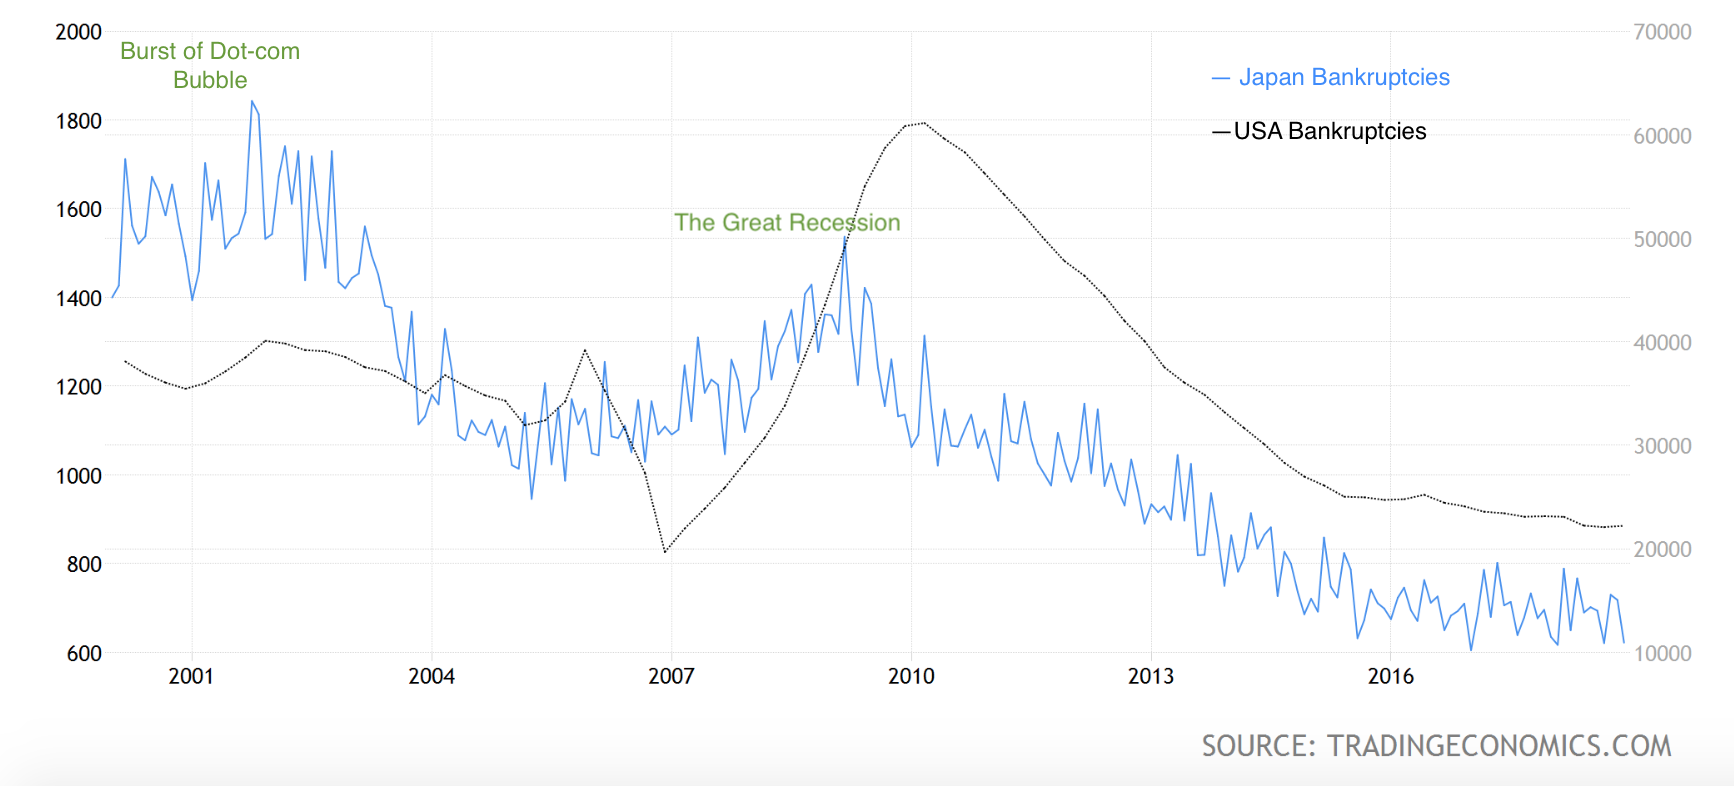
\includegraphics[height=5cm,width=\columnwidth]{Images/usaVsJapan.png}}
\caption{Comparing the number of bankruptcies in Japan and USA between 2000-2018. Source:\href{https://tradingeconomics.com/japan/bankruptcies}{ Trading Economies} }
\label{Fig:japUSA}
\end{figure}
% Location-wise, UK, Germany, France and Japan are among the leading economies in Europe and Asia. 

A comparison between Japan and the US in the number of corporate bankruptcies between 2000-2018 can be seen in \autoref{Fig:japUSA}. The figure summarises the number of bankruptcy filings each year and it is clear that the bankruptcy filing events display a strong cyclical trend. In specific, we can note the two big jumps around the most recent global recession periods, namely, the early 2000s and late 2000s. Such business-related fluctuation confirms the existence of the “domino-effect” financial distress at an international level.

In Japan, the two most prominent legal routes for filing for bankruptcy are: filing for court protection from creditors under the Corporation Reorganisation Law or under the Civil Rehabilitation Law.

The Corporation Reorganisation Law is aimed at firms whose failure would have a big impact on society, the management must resign and a new team is brought in according to a reorganisation plan devised by a court-appointed administrator. Although this procedure allows the company to sever ties with executives deemed responsible for the collapse, recovery often takes longer under this process than via the Civil Rehabilitation Law.
The Civil Rehabilitation Law, similar to America's Chapter 11, is often preferred because it allows the company to rebuild under its management team, speeding up the reconstruction process.

\section{Data-source}
\label{sec:dataSource}
We obtained the financial data of 4000 Japanese firms from an international financial database, provided by Wharton Research Data Services (\href{https://osiris.bvdinfo.com/version-20191113/home.serv?product=OsirisNeo}{Website: WRDS}). WRDS ensures convenient comparability among different countries without loss of the data consistency and reliability, regardless of differences in geometric location, business regulations etc. The database has information on listed, and major unlisted/delisted, companies across the globe. Japanese corporations also have well documented financial data as they adopt GAAP\footnote{Generally accepted accounting principles (GAAP) refer to a common set of accounting principles, standards, and procedures issued by the Financial Accounting Standards Board (FASB).} for consolidated financial statements.
% The information is very detailed and includes a lot more than financial reports.

To formally construct the international bankruptcy database, we collected each firm's annual financial information and its bankruptcy status from WRDS' annual files, this includes data from the Tokyo Stock Exchange and Osaka Securities Exchange.

% In Japan, there are six ways (including two out-of-court procedures) for a business to pursue bankruptcy proceedings. The two most prominent legal routes are: filing for court protection from creditors under the Corporation Reorganisation Law or under the Civil Rehabilitation Law.

% The Corporation Reorganisation Law is aimed at firms whose failure would have a big impact on society, the management must resign and a new team is brought in according to a reorganisation plan devised by a court-appointed administrator. Although this procedure allows the company to sever ties with executives deemed responsible for the collapse, recovery often takes longer under this process than via the Civil Rehabilitation Law.
% The Civil Rehabilitation Law, similar to America's Chapter 11, is often preferred because it allows the company to rebuild under its management team, speeding up the reconstruction process.

% When a company folds, there are two court procedures to follow: filing for bankruptcy protection or filing for special liquidation when the entity has excessive debts. 
% A company is generally deemed bankrupt if it dishonours checks twice in six months.
To maintain comparability with other studies, we have chosen to adopt the following definition of bankruptcy - a firm is classified as “bankrupt” if it files either Chapter 7 (liquidation) or Chapter 11 (using the Civil Rehabilitation Law). 
In particular, the bankruptcy indicator for the firm `i' at a time `t' is set to 1 if the firm was delisted due to filing for Chapter 7 or Chapter 11, at the time `t'. There are very few cases that firms who were delisted may re-enter the database later, but we do not consider any firm's observation after their first delisting in our analysis. 
% Companies that exit from the database for other reasons are considered as “non-bankruptcy” firms.

\subsection{Choosing 2000 to 2018 as a Sampling Period}
\label{sec:financialHistory}
In this study, we have chosen to limit our sampling period to begin from 2000 to 2018 as the Japanese economy went underwent a series of changes in bankruptcy regulations in the years leading up to 2000.
In 1998, the Japanese financial regulatory standard was tightened by the government \cite{nakamura2006japanese}. Doing so greatly weakened the original corporate structure of Japanese market - a system that mainly relied on the connection to the main bank and/or the major Keiretsu\footnote{A keiretsu is a set of companies with interlocking business relationships and shareholdings. In the legal sense, it is a type of informal business group that are loosely organised alliances within the social world of Japan's business community.} groups for financing; The research in \cite{xu2009bankruptcy} showcases this in further detail. 
Before 1998, a firm that was unable to pay off the debt from its creditors could seek financial support from the "main bank" or a certain Keiretsu group, if the company was associated to any, to avoid stepping in any further default filing process. However, after the government tightened the regulatory standard, neither the main bank nor the Keiretsu group was allowed to save a firm from default. This institutional structure change leads to an increased number of bankruptcy filings. Therefore, to avoid skewed bankruptcy figures, we begin our sampling only from 2000. 


\section{Dataset Reorganisation}
Re-organising the dataset was the most time-consuming task and the hardest challenge that we faced. The initial WRDS data set consisted of financial data from 1990 to 2018 of 4000 Japanese firms. Accounting for the reasons mentioned in the above sub-section, we first removed all the data that predated 2000. 
Our next big challenge was to combine all the available information on one timescale, as not all companies followed GAAP standards of reporting data. Careful and precise efforts needed to be undertaken to ensure that all financial indicators were reported in the same month/year so that further examinations could be made.

Acknowledging that financial data suffers from class imbalance\footnote{Our dataset consists of bankrupt and non-bankrupt/operational companies. The number of companies that go bankrupt is far fewer than the number of companies that remain operational, hence a company that goes bankrupt is part of the minority class} and concept drift\footnote{Concept drift has been explained in detail in Appendix \autoref{conceptDrift}.} that results in poor and degrading predictive performance in predictive models.  This paper proposes the use of rolling time window (as recommended in \cite{molodtsova2009out,huang2012dynamic,stock2007has}) with a fixed window size. 

% Sun \cite{sun2010dynamic} studied the mechanism of rolling time windows with fixed and variable widths, and their results showed that there was a certain degree of concept drift in financial distress prediction of Chinese listed companies. That is, under the unchanging standard definition of financial distress, incremental data would gradually take on new features of corporate financial distress in a new economic environment with time past. 

Building on the successes seen in \cite{matsunaga2019exploring,li2019dp,molodtsova2009out}, we have decided to incorporate a ten-year rolling window, to predict bankruptcy in a one-year horizon. This required us to reorganise the data to represent five forecasting years, i.e, Year 1, Year 2, Year 3, Year 4 and Year 5. This approach has been explored to outperform conventional bankruptcy models that otherwise use data from a fixed period to predict bankruptcy within a fixed horizon (number of years). \autoref{table:rolling Window} showcases the steps we have taken to reorganise the dataset, to carry out a prediction task.

\begin{table}[h!]
\begin{center}
%  \begin{tabular}{|p{2cm}|p{3cm}|p{3cm}|p{3cm}|}
 \begin{tabular}{|c|c|c|c|}
\hline
 Dataset Name & Prediction Year & Window Length & Number of Firms in Dataset 

  \\ [0.5ex] 
\hline\hline
 
Year 1 & 2013 & 2003 - 2012 & 2342  \\ \hline
Year 2 & 2014 & 2004 - 2013 & 3391  \\ \hline
Year 3 & 2015 & 2005 - 2014 & 3501  \\ \hline
Year 4 & 2016 & 2006 - 2015 & 3264  \\ \hline
Year 5 & 2017 & 2007 - 2016 & 1970  \\ 
\hline
\end{tabular}
\end{center}

    \caption{Using rolling windows to predict the bankruptcy in the next financial year.}
\label{table:rolling Window}
\end{table}


% \begin{table}[h!]
% \scriptsize
% % \captionsetup{font=normal}
% \setlength\defaultaddspace{0.66ex}
% \centering
% \begin{threeparttable}
  
%   \label{tab:history}%
%     \begin{tabular}{|l|l|l|l|}
%     \toprule
%     \textbf{Dataset Name} & \textbf{Prediction Year} & \textbf{Window Length} & \textbf{Number of Firms in Dataset}  \tabularnewline
%     \midrule
%     Year 1 & 2013 & 2003 - 2012 & 2342  \tabularnewline
% \addlinespace
%     Year 2 & 2014 & 2004 - 2013 & 3391  \tabularnewline
% \addlinespace
%     Year 3 & 2015 & 2005 - 2014 & 3501  \tabularnewline
% \addlinespace
%     Year 4 & 2016 & 2006 - 2015 & 3264  \tabularnewline
% \addlinespace
%     Year 5 & 2017 & 2007 - 2016 & 1970  \tabularnewline
% \addlinespace
    
% %     1878 & Bernard & Physiological state of cells can be maintained after the death of an organism \tabularnewline
% % \addlinespace
% %     1885 & Roux & Maintained chick embryonic cells in warm salt solutions \tabularnewline
% % \addlinespace
% %     1989 & Amgen Inc. & Recombinant erythropoietin produced in CHO cells \tabularnewline
%     \bottomrule
%     \end{tabular}%
%     \caption{Historical milestones in development of animal cell cultures (\cite{butler2004, verma2014})}
% \end{threeparttable}
% \end{table}%


\section{Dataset Description}

\subsection{Feature Extraction: Using Financial Ratios}

Studies in the past have aimed at proposing novel machine learning techniques to enhance the models’ prediction performances. However, research focused on the effect of the input variables (or features) on prediction performance is scarce.
In general, financial ratios (FRs) have been recognised as one of the most important factors affecting bankruptcy prediction and are used to develop prediction models \cite{Altman,beaver1967financial,ohlson1980financial}.

Our feature selection is based on the seminal papers \cite{Altman,beaver2005have,hardle2009variable,tian2017financial,tian2015variable, ding2012class}. A comprehensive use of financial ratios in bankruptcy prediction can be seen in the study \cite{liang2016financial}.
Financial ratios generally cover seven categories, which reflect the company’s solvency, profitability, cash flow ratios, capital structure ratios, turnover ratios, company growth and others.

%Why chosen those features
Our feature selection for this project was done by taking a tailored combination of the top eighty, most frequently occurring financial ratios that have been used in the above-mentioned papers.
% We have taken a tailored combination of the features from the above mentioned papers, based on their frequency of use and their relevancy. We chose a selection of the 100 most frequently occurring financial ratios that we deemed were important based of past literature. 
For this purpose, our Japanese dataset was re-structured to create these eighty financial ratios. In doing so, we realised that our dataset had a few limitations as it did not contain data related to the ownership structures\footnote{Ownership structure data mainly involves data related to shareholders i.e., the shareholding ratio of the board, shareholding ratio of directors, shareholding ratio of an outside person, etc.},  turnover of  `C-level' executives and compensation given to board members.
% \todo{Can be in future work - incl employee compensation}

Discarding these financial ratios, we were able to create sixty-four financial ratios that could be used as predictive variables. These synthetic features were generated by a selection of two or more existing features and applying an arithmetical operation on them. The arithmetic operation included the following set of possible values: $\{{+,-, \times,\div}\}$.

% As the focus in our project is the use of ensemble models, we use tree-based models as they have shown effective learning from the data described by many features \cite{zhou2014bankruptcy}. 

The central idea we have used in our approach is to leverage financial ratios as they may have a better influence on prediction than typical economic factors \cite{liang2016financial}. Combining financial ratios with the use of tree-based ensemble models has resulted in more effective learning from the data as shown in \cite{zhou2014bankruptcy}. We have taken advantage of this property and further propose a model that uses an ensemble of boosted trees, dedicated to solving the problem of bankruptcy prediction. 

% We can then evaluate the popularity of each feature in the forest by calculating the total number of occurrences in trees that constitutes the forest. Let us denote the total number of occurrences of
% the $d$ -th feature in the forest structure by $m_{d} .$ We define the categorical distribution $\boldsymbol{\theta}_{F}=\left[\theta_{F}^{(1)}, \cdots, \theta_{F}^{(d)}, \cdots \theta_{F}^{(D)}\right]$ for selecting the features to be
% replicated in the following manner:

% \begin{equation}
% \theta_{F}^{(d)}=\frac{m_{d}}{\sum_{d=1}^{D} m_{d}}
% \end{equation}

% As a consequence, the most popular features are going to be selected for reproduction (by the base learners in the ensemble models). The proposed procedure can be seen as a kind of an evolutionary approach that selects the strongest parents for the child feature.

The research done by Beaver, McNichols, and Rhie in \cite{beaver2005have}, on global markets, concluded that over a long period of time, the performance of the bankruptcy prediction model with both financial statement data and market data is essentially similar to the one with financial ratios only. Therefore we have considered only FRs in our model.

A description of the sixty-four features is presented in \autoref{table:FRstatsDefault}. All variables used for calculation of the financial indicators are obtained from the balance sheets, income statements or cash flow statements of the companies.


\begin{table}
\begin{center}
\small
 \begin{tabular}{|p{0.65cm}|p{6.5cm}|p{0.65cm}|p{6.5cm}|} 
\hline
 ID  & Description & ID  & Description \\ [0.5ex] 
\hline\hline
 
    X1 & Net Profit / Total Assets & X33 & Operating Expenses / Short-Term Liabilities \\ \hline

    X2 & Total Liabilities / Total Assets & X34 & Operating Expenses / Total Liabilities \\ \hline

    X3 & Working Capital / Total Assets & X35 & Profit on Sales / Total Assets \\ \hline

    X4 & Current Assets / Short-Term Liabilities & X36 & Total Sales / Total Assets \\ \hline

    X5 & [(Cash + Short-Term Securities + Receivables - Short-Term Liabilities) / (Operating Expenses - Depreciation)] * 365 & X37 & (Current Assets - Inventories) / Long-Term Liabilities \\ \hline

    X6 & Retained Earnings / Total Assets & X38 & Constant Capital / Total Assets \\ \hline

    X7 & EBIT / Total Assets & X39 & Profit on Sales / Sales \\ \hline

    X8 & Book Value of Equity / Total Liabilities & X40 & (Current Assets - Inventory - Receivables) / Short-Term Liabilities \\ \hline

    X9 & Sales / Total Assets & X41 & Total Liabilities / ((Profit on Operating Activities + Depreciation) * (12/365)) \\ \hline

    X10 & Equity / Total Assets & X42 & Profit on Operating Activities / Sales \\ \hline

    X11 & (Gross Profit + Extraordinary Items + Financial Expenses) / Total Assets & X43 & rotation Receivables + Inventory Turnover in Days \\ \hline

    X12 & Gross Profit / Short-Term Liabilities & X44 & (Receivables * 365) / Sales \\ \hline

    X13 & (Gross Profit + Depreciation) / Sales & X45 & Net Profit / Inventory \\ \hline

    X14 & (Gross Profit + Interest) / Total Assets & X46 & (Current Assets - Inventory) / Short-Term Liabilities \\ \hline

    X15 & (Total Liabilities * 365) / (Gross Profit + Depreciation) & X47 & (Inventory * 365) / Cost of Products Sold \\ \hline

    X16 & (Gross Profit + Depreciation) / Total Liabilities & X48 & EBITDA (Profit on Operating Activities - Depreciation) / Total Assets \\ \hline

    X17 & Total Assets / Total Liabilities & X49 & EBITDA (Profit on Operating Activities - Depreciation) / Sales \\ \hline

    X18 & Gross Profit / Total Assets & X50 & Current Assets / Total Liabilities \\ \hline

    X19 & Gross Profit / Sales & X51 & Short-Term Liabilities / Total Assets \\ \hline

    X20 & (Inventory * 365) / Sales & X52 & (Short-Term Liabilities * 365) / Cost of Products Sold) \\ \hline

    X21 & Sales (n) / Sales (n-1) & X53 & Equity / Fixed Assets \\ \hline

    X22 & Profit on Operating Activities / Total Assets & X54 & Constant Capital / Fixed Assets \\ \hline

    X23 & Net Profit / Sales & X55 & Working Capital \\ \hline

    X24 & Gross Profit (in 3 years) / Total Assets & X56 & (Sales - Cost of Products Sold) / Sales \\ \hline

    X25 & (Equity - Share Capital) / Total Assets & X57 & (Current Assets - Inventory - Short-Term Liabilities) / (Sales - Gross Profit - Depreciation) \\ \hline

    X26 & (Net Profit + Depreciation) / Total Liabilities & X58 & Total Costs /Total Sales \\ \hline

    X27 & Profit on Operating Activities / Financial Expenses & X59 & Long-Term Liabilities / Equity \\ \hline

    X28 & Working Capital / Fixed Assets & X60 & Sales / Inventory \\ \hline

    X29 & Logarithm of Total Assets & X61 & Sales / Receivables \\ \hline

    X30 & (Total Liabilities - Cash) / Sales & X62 & (Short-Term Liabilities *365) / Sales \\ \hline

    X31 & (Gross Profit + Interest) / Sales & X63 & Sales / Short-Term Liabilities \\ \hline
    
    X32 & (Current Liabilities * 365) / Cost of Products Sold & X64 & Sales / Fixed Assets \\ \hline
\end{tabular}
\end{center}
    \caption{Summary of features used}
\label{table:FRstatsDefault}
\end{table}


\subsection{Data Range and Correlations}
% The data ranges including the Min, Max and Mean for each financial ratio, for all 5 years can be seen in Appendix \autoref{sec:dataRange}. 

Appendix \autoref{sec:dataRange} contains the data ranges including the minimum, maximum and mean values of the financial ratios. We present the data ranges for each window (Year 1, Year 2, Year 3, Year 4 and Year5).
We have also included correlation heatmaps for the FRs in Appendix \autoref{sec:corrHeat}, examining these heatmaps, we conclude that we have a good degree of variability in our features as the heatmaps show a low correlation between features.

\subsection{Handling Missing Data}

There are three typical mechanisms causing missing data \cite{little2012prevention,sterne2009multiple,dziura2013strategies}: 
\begin{enumerate}
    \item Missing completely at random (MCAR)
    \item Missing at random (MAR)
    \item Missing not at random (MNAR)
\end{enumerate}

If the mechanism causing missing data is not dependent on observed data nor on the missing data, then data is said to be missing completely at random (MCAR) \cite{sterne2009multiple,dziura2013strategies}. MCAR causes enlarged standard errors due to the reduced sample size but do not cause bias (‘systematic error’ that is an overestimation of benefits and underestimation of harms). 
% In this situation, the incomplete data-sets are representative for the entire dataset \cite{sterne2009multiple}. More often the mechanism of missingness may depend on the observed data. If it only depends on the observed data, then the missing data are missing at random (MAR) given the observed data . 
The MAR and MNAR conditions cannot be distinguished based on the observed data since,  by definition missing data are unknown and it can therefore not be assessed if the observed data can predict the unknown data \cite{sterne2009multiple,dziura2013strategies}.


% % https://www.sciencedirect.com/science/article/pii/S095741741830616X
As justified in \cite{hosaka2019bankruptcy}, missing values in Japanese financial data could be due to the following reasons:
\begin{enumerate}
    \item The Japanese accounting standards for the net assets section changed in 2006.
    \item The notation for accounting items can differ depending on the industry, even if they have similar meanings.
    \item Items that have zero value are missing. This might cause erroneous calculations when computing financial ratios.
\end{enumerate}

Conducting further exploratory data analysis (after having created our financial ratios), we found that the dataset still contained several missing values. Examining this more closely, the dataset was tested to observe the extent of data loss if listwise deletion (an entire record is excluded from analysis if any single value is missing) is used. We observe that the data loss would be severe as we lose over 50\% of our available data. This is detailed in \autoref{table:dataLoss}

\begin{table}[h!]
% \sma
\begin{center}
 \begin{tabular}{|l|p{2.75cm}|p{2.75cm}|p{2.75cm}|p{2.75cm}|} 
 
\hline
 Dataset  & Total number of instances & Number of instances with missing data & Number of instances with no missing data & Data loss if listwise deletion is used
  \\ [0.5ex] 
 \hline\hline
 
Year 1 & 2342 & 1278 & 1064 & 54.54\% \\ \hline
Year 2 & 3391 & 2029 & 1362 & 59.81\% \\ \hline
Year 3 & 3501 & 1879 & 1628 & 53.48\% \\ \hline
Year 4 & 3264 & 1675 & 1589 & 51.29\% \\ \hline
Year 5 & 1970 & 960 & 1010 & 48.71\% \\ \hline
\hline

\end{tabular}
\end{center}

    \caption{Data Quality Assessment: Missing Data}
\label{table:dataLoss}
\end{table}

Furthermore, the python library \textbf{missingno} was used to visualise the features that had missing values. Nullity matrices were created for each forecasting period to find visual patterns of missing values; white spaces in the graph can be inferred as missing values. An example of the Year 2 dataset can be seen in \autoref{Fig:nullMatrix}

\begin{figure}[htp]
\centering
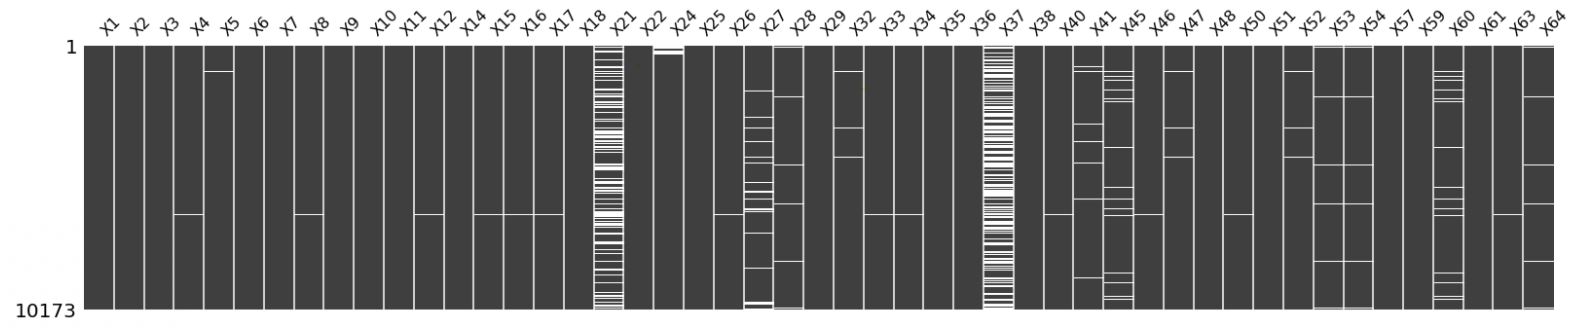
\includegraphics[height=5cm,width=1.0\columnwidth]{Images/nullityMatrix.png}
\caption{Nullity Matrix for Year 2. White space along a feature column represents missing data.}
\label{Fig:nullMatrix}
\end{figure}


In an attempt to make the data richer, we have removed all those instances that have over 50\% of their attributes as either `n.a.' or blank/empty - this resulted in our dataset shrinking by 10.3 \%. 
% This is why the number of instances is lower than expected. In doing so, the Year 5 dataset has the largest impact as the total number of available instances is reduced to 1970 as seen in \autoref{table:rolling Window}. 

Missing data can potentially cause three major problems \cite{kang2013prevention}:
\begin{enumerate}
    \item The missing data can cause bias in the estimation of parameters.
    \item It can reduce the representativeness of the samples and may complicate the analysis of the study.
    \item The absence of data reduces statistical power, which refers to the probability that the test will reject the null hypothesis when it is false.
\end{enumerate}

Dropping all the rows with missing values or listwise deletion introduces bias and affects representativeness of the results. A viable alternative to listwise deletion is by estimating missing data by using imputation techniques. In our project, we explored three techniques of imputation, and we will see them in the subsequent sections.

\begin{enumerate}
    
    
    \item Expectation-Maximisation Imputation
    \item k-Nearest Neighbours Imputation
    \item Multivariate Imputation Using Chained Equations
\end{enumerate}

% ----------------------        EM Imputation     -----------

\subsection{Expectation-Maximisation Imputation}
In statistics, Expectation–Maximisation (EM) is an iterative method to find maximum likelihood estimates of parameters in statistical models. The EM iteration alternates between performing an expectation (E) step, which creates a function for the expectation of the log-likelihood evaluated using the current estimate for the parameters. This is followed by a maximisation (M) step, which computes parameters maximising the expected log-likelihood found on the E step \cite{musil2002comparison}. 
These parameter-estimates are then used to determine the distribution of the latent variables in the next E step. 
EM Imputation is, therefore, the process of imputing missing values using Expectation-Maximisation. Missing values of quantitative variables are replaced by their expected value computed using the Expectation-Maximisation (EM) algorithm. 
In practice, a Multivariate Gaussian distribution is assumed. In general, EM imputation is better than mean imputations because they preserve the relationship with other variables \cite{ambler2007comparison}. 

We carried out EM Imputation using python's \textit{impyute} library and used 50 as the number of EM iterations to run before breaking.

% ----------------------        KNN Imputation     -----------

\subsection{k-Nearest Neighbours Imputation}

The k-nearest neighbour's algorithm or kNN is a non-parametric method used for classification and regression. In both cases, the input consists of the k closest training examples in the feature space. It can also be used as a data imputation technique where kNN imputation replaces `n.a.' and empty values in the data with the corresponding value from the nearest-neighbour row. The nearest-neighbour row is the closest row by Euclidean distance. If the corresponding value from the nearest-neighbour is also `n.a.', the next nearest neighbour is used. After finding k nearest neighbours, the weighted average of them is returned.

We carried out kNN Imputation using python's \textit{fancyimpute} library and used 100 nearest neighbours for the process.



% ----------------------        MICE Imputation     -----------

\subsection{Multivariate Imputation using Chained Equations}

\begin{figure}[htp]
\centering
\captionsetup{justification=centering}
  
  \centering
    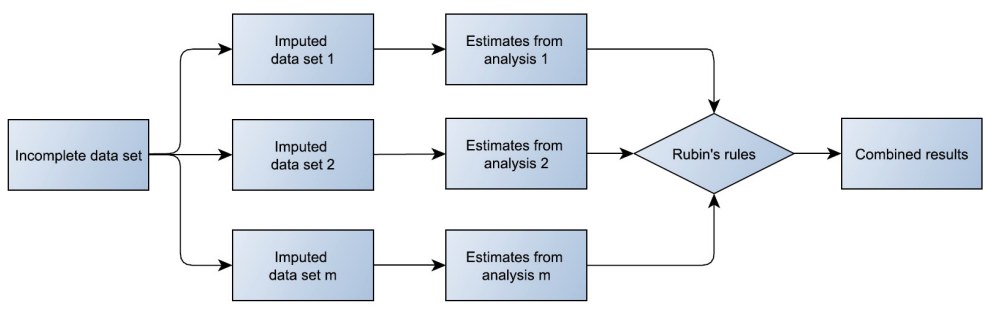
\includegraphics[width=\textwidth]{Images/Mice.png}
  \caption{The MICE-process \cite{wulff2017multiple}}
\end{figure}


Multiple imputations using chained equations or MICE is an imputation technique that uses multiple imputations to tackle missing data. MICE has become one of the principal methods of addressing missing data \cite{azur2011multiple}. Creating multiple imputations, as opposed to single imputations, accounts for the statistical uncertainty in the imputations. 

Since each variable is imputed using its own imputation model, MICE can handle different
variable types (for example, continuous, binary, categorical), as well as complexities such as varying bounds \cite{wulff2017multiple}. Multiple imputations (MI) was originally designed to handle missing data in public-use large datasets. Hence this is an ideal imputation technique for our data. 
Because multiple imputations involve creating multiple predictions for each missing value, the analysis of multiple imputed data take into account the uncertainty in the imputations and yield accurate standard errors \cite{wulff2017multiple}. 
% To carry out MICE, a series of regression models are run whereby each variable with missing data is modelled conditional upon the other variables in the data. This means that each variable can be modelled according to its distribution. For example, binary variables modelled using logistic regression and continuous variables modelled using linear regression.

We outline the MICE algorithm for a set of variables, $x_1 \dots x_k$, some or all of which have missing values. Initially, all missing values are filled in at random. The first variable with at least one missing value, $x_1$ say, is then regressed on the other variables, $x_2 \dots x_k$. The estimation is restricted to individuals with observed $x_1$. Missing values in $x_1$ are replaced by simulated draws from the posterior predictive distribution of $x_1$, an important step known as proper imputation. The next variable with missing values, say $x_2$, is regressed on all the other variables, $x_1, x_3, . . . , x_k$. Estimation is restricted to individuals with observed $x_2$ and uses the imputed values of $x_1$. Again, missing values in $x_2$ are replaced by draws from the posterior predictive distribution of $x_2$. The process is repeated for all other variables with missing values in turn: one such round is called a cycle. To stabilize the results, the procedure (similar to a Gibbs sampler) is usually repeated for about ten cycles to produce a single imputed dataset. The entire procedure is repeated independently `m' times, yielding `m' imputed data-sets. Standard texts on MI suggest that small numbers of imputed data-sets (m = 3 to 5) are adequate.


According to \cite{shrive2006dealing}, which does an extensive comparison between different imputation methods, multiple imputations is the most accurate method for dealing with missing data in most of the missing data scenarios.
The paper recommends using no more than M=5 imputations and sometimes as small number as 2 or 3 to generate useful statistical inferences. 

We carried out MICE imputation using python's \textit{fancyimpute} library and used 5 imputations in our study. 


\subsection{Dealing with Data Imbalance}
\label{sec:imbalance}
As bankruptcy is an uncommon event, it would be reasonable to note that there are only a few companies that file bankruptcy every year. We showcase this class imbalance on our own data in \autoref{table:Data organization and Instances}.

% to have a very small proportion companies in the public domain file for bankruptcy. This imbalance is evident in the dataset and is showcased in \autoref{table:Data organization and Instances}

Having an imbalanced dataset can cause our machine learning models to overfit to the majority class, i.e., companies that are still operational, i.e. non-bankrupt companies. Since the data is skewed towards one class, machine learning models can struggle to learn to correctly classify a minority class (bankrupt) instance. 
Despite this class imbalance, most models would still produce a reasonably high accuracy as most instances fall under the non-bankrupt majority class. Therefore, we disregard accuracy as a valid metric and use AUC, F1-Score, precision and recall, to evaluate the performance of our model.

To tackle this data imbalance, we use the over-sampling technique that has been proposed in \cite{le2018cluster}, to generate synthetic data that adds instances from the minority class to the dataset. This technique will raise the percentage of minority class data from around 5\% to 15\% of the dataset, as recommended by extensive work done in \cite{cao2013integrated}. This will allow the models to be exposed to a greater number of instances with the minority class, thus improving the chances for the model to predict the correct classification when an instance is labelled as bankrupt.

% In order to balance the dataset to improve the performance of the models used, we have used an oversampling technique called Synthetic Minority Over Sampling (SMOTE). The implementation and further details of this is discussed in \autoref{sec:SMOTE} 

Synthetic Minority Over-sampling Technique (SMOTE) is an algorithm has been used to over-sample the dataset as it is one of the most well-known techniques for oversampling. SMOTE \cite{chawla2002smote} works by selecting/sampling similar instances of the minority class, by finding the nearest neighbours $k$ (using Euclidean distance) and changing each attribute one at a time by multiplying each $x$ by a random number (between 0 to 1), therefore creating a new synthetic instance. We generate these minority class samples for our dataset after estimating the missing values using the previously mentioned imputation techniques. SMOTE has been implemented using the \textit{imblearn.over\_sampling} library.


\begin{table}[h!]
% \sm
\begin{center}
 \begin{tabular}{|l|p{2cm}|p{3cm}|p{3cm}|p{3cm}|} 
 \hline
 Dataset & Total number of instances & Number of bankrupt instances & Number of non-bankrupt instances & Percentage of bankrupt instances

  \\ [0.5ex] 
 \hline\hline
 
Year 1 & 2342 & 90 & 2252 & 3.93\% \\ \hline
 
Year 2 & 3391 & 134 & 3257 & 4.71\% \\ \hline
 
Year 3 & 3501 & 165 & 3336 & 5.25 \% \\ \hline
 
Year 4 & 3264 & 172 & 3092 & 6.93\% \\ \hline
 
Year 5 & 1970 & 137 & 1833 & 3.93\% \\ \hline

\end{tabular}
\end{center}

    \caption{Data organisation and Instances}
\label{table:Data organization and Instances}
\end{table}

\subsection{Dimensionality Reduction and Feature Selection}

Dimensionality reduction is a crucial component of financial analysis and has received a lot of interest in recent studies \cite{cao2012aggregating}. Many dimensionality reduction methods have been proposed, such as t-testing, correlation matrices, factor analysis, principal component analysis (PCA), independent component analysis (ICA), etc.
In a linear pre-processing stage, PCA and ICA are capable of improving the discriminating power of classifiers \cite{chen2009bankruptcy}. 
However, nonlinear projection methods are particularly applicable to solve high-dimensional financial data. Reducing the number of variables was found to be one of the key components in the successful prediction of bankruptcy, not only simplifying the model structure but also by improving the discriminative power \cite{cao2012aggregating}. The dimensionality reduction method we used is described in \autoref{sec:pca}

Feature selection techniques are methods used to eliminate features which are redundant or irrelevant. This is achieved using different methods; the most common is to find those features that are correlated to each other (or correlation with the outcome) thus removing redundant and unwanted features. 
% This in turn can simplify the hypothesis in a model which can improve both performance and memory allocation, while also reduces overfitting (reducing bias). 
Reducing the number of irrelevant or redundant features drastically reduces the running time of a learning algorithm and yields a more general concept. There are many potential benefits of feature selection, some of which are:
\begin{enumerate}
    \item Facilitating data visualisation and data understanding
    \item Reducing the measurement and storage requirements
    \item Reducing training and utilisation  times
    \item Defying the curse of dimensionality to improve prediction performances by simplifying the hypothesis in a model
\end{enumerate}

In addition, this helps in getting a better insight into the underlying concept of a real-world classification.
There are various techniques to achieve this, but for the purpose of this project, Recursive Feature Elimination (RFE) and Chi-Square feature selection will be described in \autoref{sec:RFE} and \autoref{sec:chi2} respectively.

\subsubsection{Principal Component Analysis (PCA)}
\label{sec:pca}
Dimensionality Reduction in our project was carried out using principal component analysis (PCA).
PCA re-orients a data set in the direction of the eigenvectors, which are ordered according to the extent of variance they capture from the data. The more eigenvectors we use, the higher the variance captured. PCA is a distributed representation wherein raw variables collaborate to generate a principle component. In predictive machine learning, principle components can replace the original variables. The objective is to learn the functional relationship between the target variable and the principle component. This can simplify the learning task, increase predictive accuracy, and facilitate feature reduction. 

\begin{figure}[htp]
\centering
\captionsetup{justification=centering}
  
  \centering
    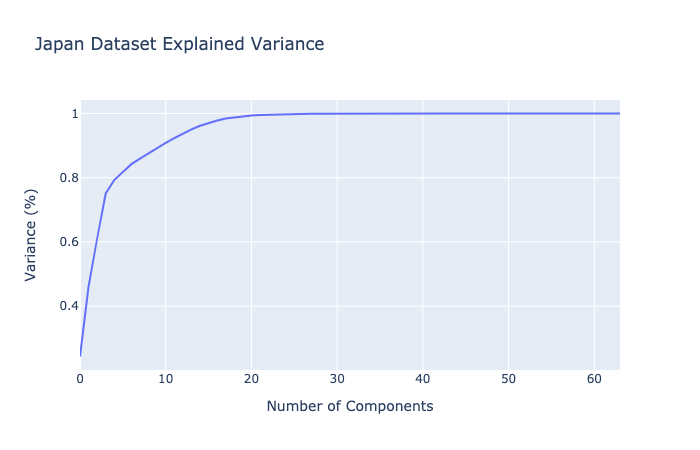
\includegraphics[width=\textwidth]{Images/pca.png}
  \caption{PCA Carried out on MICE Imputed and Oversampled Year-1 dataset.}
  \label{fig:pca}
\end{figure}

\autoref{fig:pca} shows the results of PCA being carried out on our dataset. After examining the graph, we decided to choose twenty, as the number of components as this seemed as the elbow point in the graph. Using just twenty components, we were able to attain a variance of 99.35\%.  

% \todo[inline]{New explaination}
% \textbf{COVID19-Note:} 
% The experimentation process required us to use Edinburgh University GPU's and work from DICE computers. Due to the closure of Appleton Tower on $17^{th}$ March 2020 and the inability to access University servers for computational needs, ongoing experiments using PCA was halted abruptly.
% Moving away from Edinburgh lead to further disruptions with connectivity and the change of environment demanded the need to prioritise writing the report. All further experiments were stopped due to the lack of adequate computational capacity.


\subsubsection{Recursive Feature Elimination}
\label{sec:RFE}
The Recursive Feature Elimination \cite{guyon2002gene}, as the name suggests, recursively fits the model and eliminates the least important feature/s with every iteration. This is done by ranking the features according to their coefficient weight and eliminating the least weighted features. After each iteration, the model has fitted again, and the least weighted feature/s are eliminated again until the specified number of maximum iterations or features to be eliminated is reached. In this project, the Logistic Regression classifier is used as an estimator.

The number feature selected from Recursive Feature Elimination was limited to 20, to maintain comparability with the dimensionality reduction methods.

The top 20 features selected by Recursive Feature Elimination are as follows: \\
'x11', 'x33', 'x52', 'x53', 'x61', 'x63', 'x13', 'x17', 'x19', 'x36', 'x54', 'x64', 'x6', 'x9', 'x23', 'x31', 'x32', 'x50', 'x8', 'x20'.

% \textbf{COVID19-Note:} Detailed experiments were not carried out using Chi-Square due to the lack of time and the difference seen in final results. Experimentation was halted and focus was readjusted to account new time-scale and lack of available computing resources.

\subsubsection{Chi-Square Feature Selection}
\label{sec:chi2}
The Chi-Square \cite{jin2006machine} is used to determine if the feature/s and outcome are dependent or not. The features and classes must not contain non-negative values (re-scaling is used to change negative values to positive values). It is often used in machine learning to rank features based on their Chi-Square statistic (score). Features that are found to be irrelevant for classification, are discarded depending on a specified number of features to be selected so that only the top-ranked features are selected.

Having normalised and re-scaled the data, the number feature selected from Chi-Square was limited to 20, to maintain comparability with the dimensionality reduction methods.

The top 20 features selected by Chi-Square are as follows: \\ 'x21', 'x27', 'x51', 'x32', 'x2', 'x44', 'x62', 'x43', 'x64', 'x30', 'x61', 'x52', 'x54', 'x53', 'x22', 'x58', 'x35', 'x20', 'x60', 'x47'.

\textbf{COVID19-Note:} 
The experimentation process required us to use Edinburgh University GPU's and work from DICE computers. Due to the closure of Appleton Tower on $17^{th}$ March 2020 and the inability to access University servers for computational needs, ongoing experiments using PCA, Recursive Feature Elimination and Chi-Square were halted abruptly.
Moving away from Edinburgh lead to further disruptions with connectivity and the change of environment demanded the need to prioritise writing the report. All further experiments were stopped due to the lack of adequate computational capacity.






%% ----------------------------     NEw CHAPTER BEGINS HERE ------------------------------
\chapter{Experiment Methodologies and Design}
\label{chap:Methodologies}

\section{Data Partitioning - Cross Validation}

In machine learning, model validation is referred to as the process where a trained model is evaluated with an unseen testing data set \cite{ Wang2013}. The main concept behind the validation process is to partition the dataset into a training set, which is used to train the model, and testing set, which is used to test and evaluate the model. In validation, the training set is utilised only one time, i.e., to train the model.

The problem with splitting the dataset into two partitions is that the model will only perform based on the data that was used to train it. This could lead to overfitting or underfitting hence weakening the model's ability to perform in a more generalised way ( i.e., evaluate unforeseen data outside these two partitions). Validation also tends to induce some testing bias as we reserved a piece of the dataset just for testing. To mitigate such problems and fully utilise our dataset, we use cross-validation to re-enforce the predictive ability of our model. There are various techniques which try to ensure low bias and low variances such as K-Fold Cross Validation, Stratified K-Fold Cross-Validation and Leave-P-Out Cross-Validation. 

Stratified K-Fold cross-validation has been implemented in our experiments using the python library \textit{sklearn.model\_selection.StratifiedKFold}. It is common to use this method for cross-validation as the folds are made by preserving the percentage of samples for each class.  The paper \cite{sinkey1975multivariate} discusses the benefits of using Stratified K-Fold cross-validation where there is a high disparity in the number of instances of the majority and minority class.
% Justify why this is good to do
% Stratification seeks to ensure that each fold is representative of all structure of the data. 
We ensured that each class is (approximately) equally represented across each test fold. These classes are combined in a complementary way to form training folds.

The intuition behind this relates to the bias of most classification algorithms. They tend to weight each instance equally which means over-represented classes get too much weight (e.g. optimising F1-measure, Accuracy or a complementary form of error). 
One specific issue that is important across even unbiased or balanced algorithms, is that they cannot learn or test a class that isn't represented at all in a fold {\cite{sinkey1975multivariate}}.

To carry out Stratified K-Fold cross-validation, the dataset is split into $k$ partitions, of which $k-1$ partitions are used as a training set and the one remaining partition is used as a testing set. Here we ensure that each partition has the same percentage of minority class samples as seen in that year's data. 
The process is iterated $k$ number of times so that at the end of the iterations every partition will be used once as a testing set. 
At each iteration/fold performance metrics (like AUC, F1-score, precision, recall, etc) are measured. By the end of the $k$ iterations, these metrics are averaged. This reduces both bias and variance as the original dataset is used for both training and testing sets. Therefore the model is neither overfitted by one large training set nor is it being under fitted by having a larger test set than the traditional validation method. 

This technique is applied to the different machine learning models to help in the selection of the best performing model - by using the same folds for each model at each iteration. This technique enables the facility to tune hyperparameters by using this cross-validation technique with the same model but different hyperparameters and selecting the best at the end of the iteration (using some performance metrics). We have used 10-Fold cross-validation throughout this project, similar to the approach taken in \cite{liang2016financial}.


% ----------------------        Logistic Regression     -----------


\section{Baseline with Logistic Regression}
\label{lrExplain}
The foremost method of bankruptcy prediction, proposed by Altman \cite{Altman} used logistic regression (LR). Logistic regression \cite{agresti2005bayesian} is a binary classification method which assigns one class as `1' and the second as `0' and discriminates them using a linear decision boundary. It is easy to implement and can be used as an effective baseline for binary classification problems. Being quick and effective on high-dimensional data, we use LR as a baseline classifier in this study. This model was implemented by using the python library \textit{sklearn.linear\_model.LogisticRegression}.

Logistic regression makes data assumptions such as independence and constant variance between the output and all values of the inputs. This simplicity and interpretability can occasionally lead to LR outperforming other sophisticated nonlinear models such as support vector machines \cite{kirasich2018random}, making it an effective baseline model.

In this project, LR will be utilised to classify a binary outcome (bankrupt or non-bankrupt). In this model the sigmoid function (\autoref{eqn:sigomid}) is used as a Hypothesis Function (\autoref{eqn:hypot}) to map an instance/s denoted as $x$, with some given weights denoted as $\theta$, to its Estimated Probability (\autoref{eqn:estProb}) of the discrete outcome. 
Here, $x$ represents a feature vector for observation in our data.
% Therefore, this function will output 0 ≤ hθ(x) ≤ 1 as it is shown in Figure 2.2.

\begin{equation}
\label{eqn:sigomid}
g(z)=\frac{1}{1+\exp ^{-z}}
\end{equation}

\begin{equation}
\label{eqn:hypot}
\begin{aligned}
&h_{\theta}=g\left(\theta^{T} x\right)\\
&h_{\theta}=\frac{1}{1+e^{-g\left(\theta^{T} x\right)}}
\end{aligned}
\end{equation}

The Hypothesis Function will classify an instance/s to its predicted outcome. Since the function will output the estimated probability of the discrete outcome, the model needs to interpret this output to be able to classify into `0' or `1'. To be able to compute this, a decision boundary is needed to predict $\hat{y} = 0$ or $\hat{y} = 1$, this can be seen in \autoref{eqn:yHat}. 
%  Although in most cases the threshold is set to 0.5 as explained in Condition \autoref{eqn:yHat}, in other cases this may have to be adjusted to get better results depending on the problem being tackled (threshold must always be a value between 0 and 1). The decision boundary is a property of the hypothesis, so you can have non-linear decision boundaries by adding higher polynomial terms to the features.

\begin{equation}
\label{eqn:estProb}
\begin{array}{l}
P=(\hat{y}=0 | x ; \theta)+P=(\hat{y}=1 | x ; \theta)=1 \\
P=(\hat{y}=0 | x ; \theta)=1-P=(\hat{y}=1 | x ; \theta)
\end{array}
\end{equation}

\begin{equation}
\label{eqn:yHat}
\hat{y}=\left\{\begin{array}{ll}
1 & \sigma\left(\theta^{T} x\right) \geq 0.5 ; \theta^{T} x \geq 0 \\
0 & \sigma\left(\theta^{T} x\right)<0.5 ; \theta^{T} x<0
\end{array}\right.
\end{equation}


Now that the hypothesis is defined, and the classification function is explained the model must be trained to adjust its weights $\theta$ to minimise the cost. The cost function $J(\theta)$ utilised in Logistic Regression is shown in \autoref{eqnLR:loss} and this cost function is used over the squared cost function to be able to find the global minimum when applying gradient descent. A desirable property of $J(\theta)$ is that it greatly penalises wrong predictions which have high probability with a high cost.


\begin{equation}
\label{eqnLR:loss}
J(\theta)=-\frac{1}{m} \sum_{i=1}^{m} y_{i} \log h_{\theta}\left(x_{i}\right)+\left(1-y_{i}\right) \log \left(1-h_{\theta}\left(x_{i}\right)\right)
\end{equation}

The objective is to find a set of weights such that the negative log-likelihood is minimised over the defined training set using optimisation techniques like gradient descent. The loss function (\autoref{eqnLR:loss}) measures the difference between the ground truth label and the predicted class label. If the prediction is very close to the ground truth label, the loss value is low. Alternatively, if the prediction is far from the true label, the resulting log loss will be higher.


% ---------------------- Decision Trees     -----------

\section{Decision Trees}
\label{method:DT}
A decision tree \cite{quinlan1986induction} is a learning model based on a binary tree structure. Each internal node in the tree represents a yes/no question based on a single model covariate, with the data split based on the answer. The predicted outcome of each leaf node based on the majority class of the associated samples. Decisions trees are typically learnt by considering multiple candidate covariates and split points at each internal node and selecting the one that provides the biggest increase in the homogeneity of classes in the resulting subsets.
% Decision Trees \cite{qquinlan1986induction} is a classification method that uses characteristics of the features in the dataset to build a tree of decision rules, where leaves are the different firm observations.
% Once a tree has been built from training data, an unseen data point is classified by moving down the tree, at each level choosing to descend the branch corresponding to the characteristic relevant to the data point. Eventually, a leaf node is reached, which determines the predicted class of that data point.

% The labelling process is a chain of simple decisions based on the results of sequential tests rather than a single, complex decision. Labelling involves sets of decision sequences form the branches of the decision tree, with tests being applied at the nodes. 
% Labels are assigned to terminal (leaf) nodes by means of an allocation strategy, we use majority voting. 
% Trees can be used for classification and regression \cite{quinlan1987simplifying, quinlan1986induction}.

Various algorithms can grow a tree, they differ in the possible structure of the tree (e.g.the  number of splits per node), the criteria how to find the splits, when to stop splitting and how to estimate the simple models within the leaf nodes. In this study, we have used the classification and regression trees (CART) algorithm for tree induction.

CART is a binary tree which is built by taking a set of instances from the training set and passing them to the root node, then a decision is made by using simple `if-statements', based on the features. This is done to partition the instances into two subsets and pass them as an input to child nodes. This procedure is then applied to each node until it reaches a subset with the purest (no mixed classes) distributions of the classes, known as the leaf node. 
The most important aspect of this procedure is to know which decision should be taken at each node, in order to decrease the uncertainty (minimising the mixing of classes) of the subset. Firstly, a metric to quantify the uncertainty/purity at each node is needed and in this implementation Gini Impurity \cite{breiman2017classification} is used as shown in \autoref{eqn:gini}. The formula takes the node’s class of each instance in the subset, for that node $t$, and computes the probability of obtaining two different outputs from all the possible classes $k$. If the subset only contains instances with the same label, the subset is pure, meaning $I(t) = 0$. 
% There are other methods which can be used to quantify the impurity at each node such as Entropy, MSE and MAE, but it depends on the problem being tackled (classification or regression).

\begin{equation}
\label{eqn:gini}
Gini\mbox{-}Index(t)=1-\sum_{j=1}^{k} p^{2}(j | t)
\end{equation}

A smaller Gini index value of node n represents purity, which implies that the node contains more observations from a single class. Hence, a decreasing Gini index is an important criterion for node splitting.

Additionally, another metric is needed to quantify how much a certain decision reduces uncertainty, and for this Information Gain is used. A decision is simply a condition based on a specific feature and it is usually a $\geq$ check when it's a numeric value. \autoref{eqn:IG} shows how Information Gain is computed by taking the $I(t)$ of the current node and subtracting it by the total number of samples in the right node over the total number of samples in the parent node $\frac{N_{1}^{2}}{N_{1}}$ multiplied by the right node uncertainty $I\left(t_{R}\right)$ and subtracting again with weighted average of left node uncertainty $\frac{N_{t} L}{N_{t}} I\left(t_{L}\right)$ based on a specific decision.


\begin{equation}
\label{eqn:IG}
I_{g}(t)=I(t)-\frac{N_{t R}}{N_{t}} I\left(t_{R}\right)-\frac{N_{t L}}{N_{t}} I\left(t_{L}\right)
\end{equation}


So, at each node, every feature of each instance is checked using the Information Gain to find the best split. Once this is found the node is split into two child nodes taking as input the subset which met the criteria and the subset which did not meet the criteria. This is done recursively until there is no more further splits and the leaf nodes are reached. Once the tree is built, the tree can predict the class of unseen instances by passing the test dataset to the tree. These test instances follow down the tree taking the left or right nodes based on the criteria of the decision. Once a leaf node is reached the tree will predict the probability of that instance belonging to a specific class. 
% A maximum depth for the Tree can be set or otherwise the Tree will keep on finding the best splits until all leaves are pure (if possible).


% The relationship between the class label $\hat{y}$ and features x is shown below.

% \begin{equation}
%     \hat{y} = \hat{f}(x) = \sum_{m=1}^{M}c_m I , x \in R_m
% \end{equation}

% Each instance falls into exactly one leaf node. $ I_{x \in R_m}$ is the identity function that returns 1 if $ x$ is in the subset $R_m$ and 0 otherwise. If an instance falls into a leaf node $R_l$, the predicted outcome is $\^y = c_l$  where $c_l$ is the average of all training instances in leaf node $R_l$


% This model was implemented using the python library \textbf{scikit-learn}.


%  Reasons for failing

Decision Trees are better at handling situations where the relationship between features and outcome is nonlinear or where features interact with each other (logistic regression models fail in this regard). The performance of Decision Trees although higher than LR is relatively lower compared to other ensemble techniques (as shown in \autoref{chap:results}). 
This is mainly due to two reasons \cite{dietterich2000experimental}:

\begin{enumerate}
    \item Noise present in the data.
    \item Redundant attributes of data.
\end{enumerate}

This model was implemented using the python library \textit{sklearn.tree.DecisionTreeClassifier}, with the following hyper-parameters:

\begin{enumerate}
    \item The strategy used to choose the split at each node: Best
    \item The function to measure the quality of a split: Gini
    \item The number of features to consider when looking for the best split: Number of Features

\end{enumerate}


% ----------------------        Random Forests     -----------

\section{Random Forests}
% Random forests are a popular method for classification tasks with high dimensional data. 

Random forests are ensembles of Decision Trees, the technique utilises multiple Decision Trees (weak learners) known as estimators to average out the predictions made by each tree, and this is done to reduce overfitting and to reduce the low bias, high variance trade-off found in a Decision Trees. Therefore Random forests are applied in various areas, including computer vision \cite{bosch2007image} and credit-scoring \cite{brown2012experimental},  

% because they are simple and flexible, and provide strong classification while avoiding over-fitting and improving accuracy. 

While random forests are not at the leading edge for classification tasks such as the deep learning variants technique \cite{krizhevsky2012imagenet, tanaka2017forecasting}, we choose random forests as they have several desirable features \cite{kuhn2013applied}, such as:

\begin{enumerate}
    \item Random forests provide higher discriminatory ability because they assemble the decisions of a large number of trees, instead of a single tree. 
    \item They are more generalisable and are robust to over‐fitting; hence, they may have better out‐of‐sample accuracy and be more robust to noise. 
    \item They are better at handling large datasets because they enable researchers to efficiently train multiple trees in parallel and do not require complex hyper‐parameter settings. The researchers have to choose the number of decision trees to build a model.
    
    \item They provide a measure of each variable's relative contribution to the prediction, which helps researchers identify and assess the influence of each variable while distinguishing between active and inactive companies. This can help us predict bankruptcy.
\end{enumerate}

Random Forests are very simple to use and provide high performing models without loss of interpretability, which makes them suitable for real‐world data \cite{kuhn2013applied}. 
% They are more suitable for real‐world data than are high classification performance machine learning methods like deep learning.


% An explanation of how random forests works is detailed in Appendix \autoref{explainRF}.

Predictions from random forests are made using the following process:

\begin{enumerate}
  \item Draw a subset of training data with random sampling by replacement (bootstrap).
  
  \item Train a decision tree with the subset of training data. At each node of the tree, choose the best split of a variable from only the randomly selected $m$ variables rather than from all the variables.
  
  \item Repeat steps 1 and 2 to produce $d$ decision trees.
  \item Make predictions for new data by voting for the most popular class from among all of the output of the d decision trees.
\end{enumerate}

% The Gini index (\autoref{GI}) being a popular algorithm for constructing decision trees \cite{breiman2017classification}, is also used in the base learners of random forests. 
% The algorithm selects the optimal splitting variable and the corresponding threshold value by making each node as pure as possible. Suppose $ M_n $ is the number of pieces of information reaching node n, and $ M_n^i$ is the number of data points belonging to class $ C_i$. The Gini index, $ GI_n $, of node $ n$ is thus

% \begin{equation}
% \label{GI}
%     GI_n = 1 - \sum_{i=1}^{K} (p_n^i)^2,  \hbox{where }  p_n^i = M_n^i / M_n
% \end{equation}

% A smaller Gini index value of node n represents purity, which implies that the node contains more observations from a single class. Hence, a decreasing Gini index is an important criterion for node splitting.

This model was implemented using the python library \textit{sklearn.ensemble.RandomForestClassifier}, with the following hyper-parameters mentioned below:

\begin{enumerate}
    \item The number of trees in the forest = 100
    \item The function to measure the quality of a split: Gini
    \item The number of features to consider when looking for the best split: $\sqrt{Number\mbox{ }of\mbox{ }Features}$

\end{enumerate}

% ----------------------        Balanced Bagging Classifier     -----------

\section{Bagging}
Breiman’s bagging \cite{breiman1996bagging}, also known as bootstrap aggregating, is one of the earliest ensemble learning algorithms. It is a technique involving independent classifiers that uses portions of the data and then combines them through model averaging, providing efficient results concerning a collection. It is designed to improve the stability and accuracy of classification \cite{quinlan1987simplifying} while simultaneously reducing variance to avoid overfitting.

Diversity in bagging is obtained by using bootstrapped replicas of the training dataset, i.e., different training data subsets are randomly drawn—with replacement—from the entire training dataset. Each training data subset is used to train a different base learner of the same type. The base learners’ combination strategy for bagging is a majority vote. This simple strategy can reduce variance (hence prevent overfitting) when combined with the base learner generation strategies \cite{figini2016corporate}. 


We have implemented the bagging algorithm as follows:

\begin{enumerate}
    \item A random bootstrap set, $t$, is selected from the parent dataset.
    \item Classifiers $C_{t}$ are configured on the dataset from step $1 .$
    \item Steps 1 and 2 are repeated for $t=1, \ldots, T$
    \item Each classifier determines a vote based on : 
$C(x)=T^{-1} \sum_{t=1}^{T} C_{t}(x)$
\\where x is the data of each element from the training set. In the last step, the class that receives the largest number of votes is chosen as the classifier for the dataset.
\end{enumerate}


This model was implemented using the python library \textit{imblearn.ensemble.BalancedBaggingClassifier}, with the following hyper-parameters mentioned below:

\begin{enumerate}
    \item The number of base estimators in the ensemble = 5
    \item Base Learner = Random Forests
    \item Bootstrap = True
\end{enumerate}

% ---------------------         XGBOOST         ----------------------------

\section{Extreme Gradient Boosting Classifier (XGBoost)}
% ------------Why?
XGBoost was chosen as a suitable model as it provides a strong regularisation framework that constrains overfitting \cite{sewell2008ensemble}. The algorithm was developed to efficiently reduce computing time and allocate an optimal usage of memory resources. As mentioned in \cite{chen2016xgboost}, important features of implementation include:
\begin{enumerate}
    \item Handling of missing values (Sparse Aware).
    \item Block Structure to support parallelisation in tree construction.
    \item The ability to fit and boost new data added to a trained model (Continued Training).
    
\end{enumerate}

As an ensemble tree-boosting method, XGBoost predicts a new classification membership after each iteration. This is done in an additive way, i.e., that predictions are made from weak classifiers, that constantly improve over the previous classifier's error. Incorrectly classified samples receive higher weights at the next step, forcing the classifier to focus on their performance in the following iterations. The final classification is vigorous as it includes the combined improvement of all the previous modelled trees. The learning of these classifiers is based on defining an objective function \cite{chen2015xgboost}. This function represents training loss and regularisation. The former describes the predictive accuracy of the model, while the latter describes the complexity. The working of XGBoost is now discussed in detail.

Let us denote by $\mathbf{x} \in \mathscr{X}$ a vector of features describing an enterprise, where $X \subseteq \mathbb{R}^{D}$ and by $y \in\{0,1\}$ a label representing whether the enterprise is bankrupt, $y=1$, or not, $y=0$. Further, we utilise Decision Trees as discriminative models, specifically, we use CART. A CART tree can be represented by the weights associated with the leaves in the tree structure

\begin{equation}
f_{k}\left(\mathbf{x}_{n}\right)=w_{q(\mathbf{x})}
\end{equation}

where $q\left(\mathbf{x}_{n}\right)$ is the function that takes an example $\mathbf{x}$ and returns the path id in the structure of the tree, $q: \mathbb{R}^{D} \rightarrow\{1, \cdots, T\},$ T is the number of paths (leaves). A path is ended with a leaf that contains weight $w_{i}$

Our algorithm aims at learning an ensemble of $K$ decision trees \cite{chen2015xgboost} as shown below.

\begin{equation}
h_{K}(\mathbf{x})=\sum_{k=1}^{K} f_{k}(\mathbf{x})
\end{equation}

where $f_{k} \in \mathscr{F},$ for $k=1, \dots, K,$ and $F$ is a space of all possible decision trees (CART). To obtain a decision for new x, the conditional probability of a class for $h_K$ is calculated as follows:

\begin{equation}
p(y=1 | \mathbf{x})=\sigma\left(h_{K}(\mathbf{x})\right)
\end{equation}

where sigma is the sigmoid function (seen in \autoref{eqn:sigomid}).
For given training data $\mathscr{D}=\left\{\mathbf{x}_{n}, y_{n}\right\}_{n=1}^{N},$ the model is trained by minimising the following criterion:

\begin{equation}
\label{eqn:xgbProb}
\begin{aligned}
L_{\Omega}(\boldsymbol{\theta}) &=L(\boldsymbol{\theta})+\Omega(\boldsymbol{\theta}) \\
&=\sum_{n=1}^{N} l\left(y_{n}, h_{K}\left(\mathbf{x}_{n}\right)\right)+\sum_{k=1}^{K} \Omega\left(f_{k}\right)
\end{aligned}
\end{equation}

The ensemble model for this loss function is known as the Logit-Boost model \cite{chen2015xgboost}.

The problem of learning such model can be solved iteratively by adding a new weak learner $f_{k}(.)$ in the $k^{th}$  training iteration assuming that models $f_{1}(\cdot), \cdots, f_{k-1}(\cdot)$ are already trained. We can present the loss function for single example $l\left(y_{n}, h_{k}\left(\mathbf{x}_{n}\right)\right)$ in the following manner:

\begin{equation}
l\left(y_{n}, h_{k}\left(\mathbf{x}_{n}\right)\right)=l\left(y_{n}, h_{k-1}\left(\mathbf{x}_{n}\right)+f_{k}\left(\mathbf{x}_{n}\right)\right)
\end{equation}

We assumed an additive regularisation term, therefore we can represent it in the following form:

\begin{equation}
L_{\Omega}(\boldsymbol{\theta})=\sum_{n=1}^{N} l\left(y_{n}, h_{k-1}\left(\mathbf{x}_{n}\right)+f_{k}\left(\mathbf{x}_{n}\right)\right)+\Omega\left(f_{k}\right)+\text { constant }
\end{equation}

Therefore, we can represent the general learning criterion (\autoref{eqn:xgbProb}) as:

\begin{equation}
\label{eqn:xgb14}
L_{\Omega}(\boldsymbol{\theta})=\sum_{n=1}^{N} l\left(y_{n}, h_{k-1}\left(\mathbf{x}_{n}\right)+f_{k}\left(\mathbf{x}_{n}\right)\right)+\Omega\left(f_{k}\right)+\text { constant }
\end{equation}

Further, approximating the objective function using the Taylor expansion with respect to $h_{k-1}\left(\mathbf{x}_{n}\right)$ yields the following:

\begin{equation}
\begin{aligned}
L_{\Omega}(\boldsymbol{\theta}) & \simeq \sum_{n=1}^{N}\left[l\left(y_{n}, h_{k-1}\left(\mathbf{x}_{n}\right)\right)+g_{n} \cdot f_{k}\left(\mathbf{x}_{n}\right)+\frac{1}{2} \cdot h_{n} \cdot f_{k}^{2}\left(\mathbf{x}_{n}\right)\right] \\
&+\Omega\left(f_{k}\right)+\text { constant }
\end{aligned}
\end{equation}

where $g_{n}$ is the first derivative with respect to $h_{k-1}\left(\mathbf{x}_{n}\right)$

\begin{equation}
g_{n}=\frac{\partial l\left(y_{n}, h_{k-1}\left(\mathbf{x}_{n}\right)\right)}{\partial h_{k-1}\left(\mathbf{x}_{n}\right)}
\end{equation}

and $h_{n}$ is the second derivative with respect to $h_{k-1}\left(\mathbf{x}_{n}\right)$

\begin{equation}
h_{n}=\frac{\partial^{2} l\left(y_{n}, h_{k-1}\left(\mathbf{x}_{n}\right)\right)}{\partial h_{k-1}^{2}\left(\mathbf{x}_{n}\right)}
\end{equation}


Considering the logistic loss (\autoref{eqn:xgbProb}), $g_n$ can be re-written as:

\begin{equation}
\begin{aligned}
g_{n} &=-y_{n} \frac{\exp \left\{-h_{k-1}\left(\mathbf{x}_{n}\right)\right\}}{1+\exp \left\{-h_{k-1}\left(\mathbf{x}_{n}\right)\right\}}+\left(1-y_{n}\right) \frac{\exp \left\{h_{k-1}\left(\mathbf{x}_{n}\right)\right\}}{1+\exp \left\{h_{k-1}\left(\mathbf{x}_{n}\right)\right\}} \\
&=-y_{n} \frac{1}{1+\exp \left\{h_{k-1}\left(\mathbf{x}_{n}\right)\right\}}+\left(1-y_{n}\right) \frac{1}{1+\exp \left\{-h_{k-1}\left(\mathbf{x}_{n}\right)\right\}} \\
&=-y_{n}\left(1-\sigma\left(h_{k-1}\left(\mathbf{x}_{n}\right)\right)\right)+\left(1-y_{n}\right) \sigma\left(h_{k-1}\left(\mathbf{x}_{n}\right)\right) \\
&=\sigma\left(h_{k-1}\left(\mathbf{x}_{n}\right)\right)-y_{n}
\end{aligned}
\end{equation}


In calculating the first derivative we took advantage of the sigmoid function property, namely, $\sigma(-a)=1-\sigma(a) .$ It can be observed, that $\sigma\left(h_{k-1}\left(\mathbf{x}_{n}\right)\right)$ has interpretation of the probability of observing the class indexed by 1 for the example $\mathbf{x}_{n}$

We can make use of $\sigma^{\prime}(a)=\sigma(a)(1-\sigma(a))$ property to calculate the second derivative, $h_{n}$.

\begin{equation}
h_{n}=\sigma\left(h_{k-1}\left(\mathbf{x}_{n}\right)\right)\left(1-\sigma\left(h_{k-1}\left(\mathbf{x}_{n}\right)\right)\right)
\end{equation}

There are different possible regularisation terms. However, in our considerations we focus on the regulariser in the following form:

\begin{equation}
\Omega\left(f_{k}\right)=\gamma T+\frac{1}{2} \lambda \sum_{t=1}^{T} w_{t}^{2}
\end{equation}

where $\lambda$ and $\gamma$ are the parameters of the regularisation term. For the tree representation with weights the objective function given in (\autoref{eqn:xgb14}) can be presented in the following manner:

\begin{equation}
\begin{aligned}
L_{\Omega}(\boldsymbol{\theta}) & \simeq \sum_{n=1}^{N}\left[g_{n} w_{q\left(\mathbf{x}_{n}\right)}+\frac{1}{2} h_{n} \cdot w_{q\left(\mathbf{x}_{n}\right)}^{2}\right]+\gamma T \\
&+\frac{1}{2} \lambda \sum_{t=1}^{T} w_{t}^{2}+\text { constant } \\
&=\sum_{t=1}^{T}\left[\left(\sum_{j \in I_{I}} g_{j}\right) w_{t}+\frac{1}{2}\left(\sum_{j \in I_{t}} h_{j}+\lambda\right) w_{t}^{2}\right]+\gamma T+\text { constant } \\
&=\sum_{t=1}^{T}\left[G_{t} w_{t}+\frac{1}{2}\left(H_{t}+\lambda\right) w_{t}^{2}\right]+\gamma T+\text { constant }
\end{aligned}
\end{equation}

where $I_{t}=\left\{n | q\left(\mathbf{x}_{n}\right)=t\right\}$ is the set of indexes of instances associated with the $t$ -th leaf in the tree, $G_{t}=\sum_{j \in I_{t}} g_{j}$ and $H_{t}=\sum_{j \in I_{t}} h_{j} .$ Assuming the known structure of the tree, the optimal value of the weight in the $t-$ th leaf is as follows:


\begin{equation}
w_{t}^{*}=-\frac{G_{t}}{H_{t}+\lambda}
\end{equation}

The optimal value of the approximated objective function is given by

\begin{equation}
L_{\Omega}(\boldsymbol{\theta}) \simeq-\frac{1}{2} \sum_{t=1}^{T} \frac{G_{t}^{2}}{H_{t}+\lambda}+\gamma T+\text { constant }
\end{equation}


The key problem in the above consideration is that the structure of the tree is not given in advanced and searching all possible structures is computationally not feasible. To overcome this issue the tree is being constructed starting from the root. Further, the best attribute located in the root is selected and the best split point for the attribute is chosen. The splitting process is performed until the quality of the model is improved. As the splitting criterion we take the Information Gain:

\begin{equation}
\label{eqn:Gain}
\mathscr{Gain}=\frac{G_{L}^{2}}{H_{L}+\lambda}+\frac{G_{R}^{2}}{H_{R}+\lambda}-\frac{\left(G_{L}+G_{R}\right)^{2}}{H_{R}+H_{L}+\lambda}-\gamma
\end{equation}

where $\frac{G_{L}^{2}}{H_{L}+\lambda}$ is the score value calculated for the left child, $\frac{G_{R}^{2}}{H_{R}+\lambda}$ for is the score value for the right ancestor and $\frac{\left(G_{L}+G_{R}\right)^{2}}{H_{R}+H_{L}+\lambda}$ is the score value if splitting is not performed. Parameter $\gamma$ penalizes addition of more leaves to the tree structure.
The model can be also regularised by setting a minimum number of examples combined with each of the leaves, by setting the maximal depth of the tree, by setting the percentage of features randomised for each iteration of constructing the tree or by adding the new tree with the corrected influence of the trees in the committee

\begin{equation}
h_{k}\left(\mathbf{x}_{n}\right)=h_{k-1}\left(\mathbf{x}_{n}\right)+\epsilon f_{k}\left(\mathbf{x}_{n}\right)
\end{equation}

where $\epsilon \in[0,1]$ is called step-size or shrinkage.


% % \label{explain:XGB}
% Chen and Guestrin \cite{chen2016xgboost} describe XGBboost as an ensemble of K Classification and Regression Trees (CART) \(\left\{T_{1}\left(x_{i}, y_{i}\right), \ldots . T_{K}\left(x_{i}, y_{i}\right)\right\}\) where \(x_{i}\) is the given training set of descriptors associated with a molecule to predict the class label, y, Given that CART assigns a real score to each leaves (outcome or target), the prediction scores for individual CART is summed up to get the final score and evaluated through \(K\) additive functions, as shown in  \autoref{xgb1}:

% \begin{equation}
% \label{xgb1}
% \hat{y}_{i}=\sum_{k=1}^{K} f_{k}\left(x_{i}\right), f_{k} \in F
% \end{equation}

% where \(f_{k}\) represents an independent tree structure with leaf scores and \(F\) is the space of all CART. The regularized objective to optimize is given by  \autoref{xgb2}:

% \begin{equation}
% \label{xgb2}
% \operatorname{Obj}(\Theta)=\sum_{i}^{n} l\left(y_{i}, \hat{y}_{i}\right)+\sum_{k}^{K} \Omega\left(f_{k}\right)
% \end{equation}

% The first term is a differentiable loss function, \(l,\) which measures the difference between the predicted \(\hat{y}\) and the target \(y_{i}\). The second is a regularization term \(\Omega\) which penalizes the complexity of the model to avoid overfitting. It is given by \(\Omega(f)= \alpha T+\frac{1}{2} \lambda \sum_{j-1}^{T} w_{j}^{2}\), where \(T\) and \(w\) are the number of leaves and the score on each leaf respectively.  $\alpha$ and $\lambda$ are constants to control the degree of regularization. Apart from the use of regularization, shrinkage and descriptor subsampling are two additional techniques used to prevent overfitting \cite{sewell2008ensemble}.



% Training XGBoost is summarized as follows:

% \begin{enumerate}
%     \item For each descriptor:
%         \begin{enumerate}
%                 \item Sort the numbers
%                 \item Scan the best point to split, i.e, the lowest gain
%         \end{enumerate}
      
%     \item Choose the descriptor with the best splitting point that optimizes the training objective
%     \item Continue splitting (as in (Step 1) and (Step 2)) until the specified maximum tree depth is reached
%     \item Assign prediction score to the leaves and prune all negative nodes (nodes with negative gains) in a bottom-up order
%     \item Repeat the above steps in an additive manner until the specified number of rounds (trees K) is reached.
% \end{enumerate}


% Since additive training is used, the prediction $\hat{y}$ at step $t$ expressed as

% \begin{equation}
% \hat{y}_{i}^{(t)}=\sum_{k=1}^{K} f_{k}\left(x_{i}\right)=\hat{y}_{i}^{(t-1)}+f_{t}\left(x_{i}\right)
% \end{equation}

% And the objective function can be written as:

% \begin{equation}
% \operatorname{Obj}(\Theta)^{(t)}=\sum_{i}^{n} l\left(y_{i}, \hat{y}_{i}^{(t-1)}+f_{t}\left(x_{i}\right)\right)+\Omega\left(f_{t}\right)
% \end{equation}
\begin{table}[h!]
\begin{center}
 \begin{tabular}{ | p{3cm}| p{3cm} | p{3cm} | p{3cm}|}
 \hline
  Parameter & Domain & Default Parameter & After Tuning

  \\ [0.5ex] 
 \hline\hline
n\_estimators & (100,500)& 100.0 & 100 \\ \hline
max\_depth & (5,30) & 3.0 & 9.0 \\ \hline
learning\_rate & (0.005,0.2) & 0.1 & 0.2 \\ \hline
min\_child\_weight & (1,50) & 1.0 & 14.0 \\\hline
subsample & (0.8,1.0) & 1.0 & 1.0 \\\hline
colsample\_bytree &(0.8,1.0 ) &1.0 & 1.0 \\\hline
 colsample\_bylevel &(0.8,1.0 ) &1.0 & 1.0 \\\hline
gamma & (0,0.02)&0.0 & 0.0 \\\hline

\end{tabular}
\end{center}

    \caption{XGBoost Hyper-Parameters}
\label{table:XBG_setting}
\end{table}


This model was implemented using the python library \textit{xgboost.XGBClassifier}. The domain of hyper-parameters was taken from those suggested in
\cite{wang2019xgboost}. 
Starting with the default, we carried out a  grid search of the parameters in that domain to obtain the best hyper-parameters for our task. This can be seen in \autoref{table:XBG_setting}.
% \begin{enumerate}
%     \item Learning Rate = 0.01
%     \item Objective = Binary:logistic
%     \item Number of gradient boosted trees = 100
%     \item Maximum tree depth for base learners = 4

% \end{enumerate}



\section{Model Evaluation}
\label{sec:modelEval}
In accordance with 2019's Basel III\footnote{Basel III is an international regulatory accord that introduced a set of reforms designed to improve the regulation, supervision and risk management within the banking sector.} 
regulations for evaluating bankruptcies and default models, it is crucial to choose a bankruptcy prediction model that scores well on a range of different performance metrics. 

The accuracy measure of a model is not well-suited for imbalanced datasets and they can be largely ignored in a dataset where a large proportion of the observations belong to one class. The issue with the accuracy measure is that it does not look at class breakdown precision, nor does it provide evidence of true positives or true negatives values. 
% The false positive rate, on its own, serves a somewhat limited role in this study as well. It is primarily used as validation metric to ensure that the trained model, from which the variable importance measure is derived, does not mistakenly predict healthy firms as being bankrupt (false positives) as this would undermine the validity of the variable importance measures and resulting variable ranking.

To conduct a credible performance evaluation that accounts for overfitting and generalisability, we measure the following metrics on each model:
\begin{enumerate}
    \item Precision
    \item Recall
    \item F1-Score
    \item Area under the Receiver Operating Characteristics (ROC) curve
    
\end{enumerate}

\subsection{Precision}
Precision is as defined as the proportion of positive identifications that are actually correct (\autoref{eqn:precision}). High Precision indicates an instance when labelled as positive is indeed positive (a small number of false positives).
In our task, a high precision value indicates an instance that is classified to be bankrupt, is actually bankrupt.

\begin{equation}
\label{eqn:precision}
    Precision = \frac{True\mbox{-}Positive }{True\mbox{-}Positive + False\mbox{-}Positive}
\end{equation}

\subsection{Recall}
Recall (Sensitivity) is defined as the proportion of actual positives that have been identified correctly (\autoref{eqn:recall}). High Recall indicates that the class is correctly recognised (a small number of false negatives).
The question recall address is: Of all the companies that have gone bankrupt, how many did the model label? 

% Recall is used when we want to mostly focus on false-negative i.e to decrease false negative value thereby increase recall value.

\begin{equation}
\label{eqn:recall}
    Recall = \frac{True\mbox{-}Positive }{True\mbox{-}Positive + False\mbox{-}Negative}
\end{equation}

\subsection{F1-Score}
F1-score is a good performance metrics that leverages both precision and recall metrics. F1-score is obtained by taking the harmonic mean in place of arithmetic mean as it punishes the extreme values more.
Unlike precision which mostly focuses on false-positive and recall which mostly focuses on false-negative, F1-score is a feasible metric that accounts for both false positive and false negative rates. 
% F1-Score is used when we want to penalise both false-negatives and false-positives by hoping to decrease them in order to increase F1-Score.

\begin{equation}
\label{eqn:recall}
    F1\mbox{-}Score = 2 \times \frac{Precision \times Recall}{Precision + Recall}
\end{equation}

\subsection{Area Under the Curve (AUC)}
The receiver operating characteristic curve (ROC) is a plot of the true positive rate (TPR) versus the false positive rate (FPR) for the predictions of a binary classifier at multiple thresholds. The integrated area under the curve (AUC ROC) provides a summary measure of the discriminative ability of the model across all evaluated thresholds. AUC is desirable for the following two reasons:
\begin{enumerate}
    \item AUC is scale-invariant. It measures how well predictions are ranked, rather than their absolute values.
    \item AUC is classification-threshold-invariant. It measures the quality of the model's predictions irrespective of what classification threshold is chosen.
\end{enumerate}

Since performance is evaluated at multiple thresholds, AUC ROC is less sensitive to imbalanced class distributions compared to other commonly reported metrics ( e.g. Accuracy, TPR, True Negative Rate (TNR)) making it suitable for this task \cite{bradley1997use}.
The AUC of the ROC curve corresponds to the value of the WilcoxonMann-Whitney test, it is used as a measure of `goodness' for predictions \cite{vihinen2012evaluate}. The range of AUC ROC values is between 0.5 and 1.0 with a value of 0.5 representing a classifier that is no better than randomly guessing the class and a value of 1.0 signifying a classifier with perfect discriminative ability.




%% --------------------------       NEW CHAPTER BEGINS HERE         ------------------------------
\chapter{Empirical Results}
\label{chap:results}
\label{chap:Results}

We repeated 10-fold cross-validations for five times with different random seeds as is conducted by \cite{kim2010ensemble} in order to ensure that the comparison among three different classifiers does not happen by chance. For each of 10-fold cross-validation, the entire data set is first partitioned into 10 equal-sized sets, and then each set is in turn used as the test set while the classifier trains on the other nine sets. The cross-validated folds were tested independently of each algorithm. This way we obtained the results for four classifiers (and the baseline) on each of the fifty experiments. The empirical results reported in this section are the averages of the evaluation metrics used.
% The empirical results consists of the performance of the four classifiers using three different imputation techniques. We evaluate these classifiers on four performance metrics discussed in \autoref{sec:modelEval}.

\section{Baseline Results}
We began our initial experiments by setting a valid baseline. We followed Altman's \cite{Altman} footsteps and used Logistic Regression (LR) as our baseline classifier. \autoref{table:Baseresults} shows the results obtained. Examining these results, we make the following observations;
first when data is not imputed LR performs worse than a random classifier. This is because LR is not good at handling missing data and performs poorly when it is not accounted for.
Second, incorporating imputation techniques but leaving out the oversampling step brings about a significant increase (over 10\%) in the AUC score. These models suffer from a low precision score suggesting that there are many false positives in the model.
Third, the ideal baseline results are produced when both imputation and oversampling are used, particularly when kNN imputation is used. \textbf{This is our best performing baseline with an AUC score of 0.628 and an F1-score of 0.564.}


\begin{table}[htp]
\small
\begin{center}
 \begin{tabular}{ | p{2cm} | p{1.5cm} | p{2cm} | p{1.5cm}| p{1.5cm} | p{1.5cm}| p{1.5cm} | }
 \hline
  Model & Imputation & Oversampled & Precision  & Recall & F1-Score & AUC

  \\ [0.5ex] 
 \hline\hline

    Logistic Regression & None & No& 0.044 & 0.030 & 0.036 & 0.448 \\ \hline
    Logistic Regression & None & Yes& 0.053 & 0.035 & 0.042 & 0.473 \\ \hline
    \midrule
    Logistic Regression & EM & No & 0.064 & 0.360 & 0.108 & 0.583 \\ \hline
    Logistic Regression & KNN & No & 0.068 & 0.370 & 0.115 & 0.592\\ \hline
    Logistic Regression & MICE & No & 0.068 & 0.370 & 0.115 & 0.592  \\ \hline
    \midrule
    Logistic Regression & EM & Yes & 0.515 & 0.490 & 0.503 & 0.580 \\ \hline
    \textbf{Logistic Regression} & \textbf{KNN} & \textbf{Yes} & \textbf{0.570} & \textbf{0.559} & \textbf{0.564} & \textbf{0.628}\\ \hline
    Logistic Regression & MICE & Yes & 0.504 & 0.647 & 0.567 & 0.595  \\ \hline

\end{tabular}
\end{center}

    \caption{Baseline Results}
\label{table:Baseresults}
\end{table}

%-----------------------------------------------------------------------------------------------------

\section{Results from Machine Learning Models}


% ------noSMOTEnoImputation ------
\autoref{table:noSMOTEnoImputation} shows the results we obtained, solely by applying our classifiers on the raw data, i.e., without imputing the data nor oversampling the minority class. As expected, the performance of our classifiers is very poor, this is evident from the low F1 and AUC scores. As the AUC scores are just over 0.5, these models are only marginally better than a random classification.

\begin{table}[h!]
\begin{center}
 \begin{tabular}{ | p{3cm} | p{2cm} | p{1.75cm}| p{1.75cm} | p{1.75cm}| p{1.75cm} | }
 \hline
  Model & Imputation &  Precision  & Recall & F1-Score & AUC

  \\ [0.5ex] 
 \hline\hline
    
    Decision Tree & None & 0.070 & 0.120 & 0.088 & 0.507 \\ \hline
    Random Forest & None & 0.102 & 0.251 & 0.145 & 0.512 \\ \hline
    Bagging & None & 0.017 & 0.556 & 0.033 & 0.563 \\ \hline
    XGBoost & None & 0.050 & 0.032 & 0.039 & 0.527 \\ \hline
    
\end{tabular}
\end{center}

    \caption{Experiment results without data imputation nor minority class oversampling.}
\label{table:noSMOTEnoImputation}
\end{table}


% --------------table:yesImputenoSMOTE

Following this, we incorporate the imputation techniques to estimate the missing values present in our data.
\autoref{table:yesImputenoSMOTE} shows the results obtained by the classification models. 
We see that all the classifiers seem to be involved in a 'tug-of-war' match between precision and recall values.

A high recall, the low precision value indicates that most of the positive examples are correctly recognised (low false negatives) but there are a lot of false positives. This is seen in the Bagging ensemble model that achieves an AUC score of 0.746 with MICE imputation.
Whereas a low recall value, high precision indicates that the model misses a lot of positive examples (high false negatives) but those we predicted as positive are indeed positive (low false positives). This can be observed in the Random Forests with MICE imputation model that achieves an AUC score of 0.739.


\begin{table}
\begin{center}
 \begin{tabular}{ | p{3cm} | p{2cm} | p{1.75cm}| p{1.75cm} | p{1.75cm}| p{1.75cm} | }
 \hline
  Model & Imputation &  Precision  & Recall & F1-Score & AUC

  \\ [0.5ex] 
 \hline\hline

    Decision Tree & EM & 0.361 & 0.520 & 0.426 & 0.701 \\ \hline
    Decision Tree & KNN & 0.414 & 0.550 & 0.472 & 0.721 \\ \hline
    Decision Tree & MICE & 0.384 & 0.530 & 0.445 & 0.709 \\ \hline
    Random Forest & EM & 0.800 & 0.080 & 0.145 & 0.540 \\ \hline
    Random Forest & KNN & 0.650 & 0.130 & 0.217 & 0.563 \\ \hline
    Random Forest & MICE & 0.894 & 0.420 & 0.572 & 0.739 \\ \hline
    Bagging & EM & 0.121 & 0.670 & 0.205 & 0.705 \\ \hline
    Bagging & KNN & 0.149 & 0.660 & 0.243 & 0.721 \\ \hline
    Bagging & MICE & 0.171 & 0.770 & 0.280 & 0.746 \\ \hline
    XGBoost & EM & 0.881 & 0.370 & 0.521 & 0.684 \\ \hline
    XGBoost & KNN & 0.933 & 0.420 & 0.579 & 0.709 \\ \hline
    XGBoost & MICE & 0.945 & 0.520 & 0.671 & 0.759 \\ \hline
\end{tabular}
\end{center}

    \caption{Experiment results when data is imputed but not oversampled.}
\label{table:yesImputenoSMOTE}
\end{table}

% ----------------


% table:noImputeyesSmote-------------

Next, we used SMOTE to oversample the minority class and to examine the effect that this process would have without performing data imputations. From \autoref{table:noImputeyesSmote} we note that the results are an improvement when compared to the experiment setup in  \autoref{table:noSMOTEnoImputation}; but the overall performance of these classifiers is still poor. The low precision and recall values indicate that the model still suffers from high false-positive and high false-negative rates.

\begin{table}[htpb]
\begin{center}
 \begin{tabular}{ | p{3cm} | p{2cm} | p{1.75cm}| p{1.75cm} | p{1.75cm}| p{1.75cm} | }
 \hline
  Model & Imputation &  Precision  & Recall & F1-Score & AUC

  \\ [0.5ex] 
 \hline\hline
    
    Decision Tree & None & 0.084 & 0.138 & 0.104 & 0.684 \\ \hline
    Random Forest & None & 0.122 & 0.289 & 0.172 & 0.691 \\ \hline
    Bagging & None & 0.020 & 0.639 & 0.040 & 0.760 \\ \hline
    XGBoost & None & 0.060 & 0.037 & 0.046 & 0.711 \\ \hline
    
\end{tabular}
\end{center}

    \caption{Experiment results from oversampling the minority class to 15\% of the data.}
\label{table:noImputeyesSmote}
\end{table}
% -----------------

\section{The Best Model}

Finally, we combined the use of imputation techniques and oversampling of the minority class.  \autoref{table:results} showcases a significant improvement across all the performance metrics.
The combination of MICE imputation and oversampling achieves the highest performance amongst all the classifiers used.
We conclude our experiments by reporting that XGBoost, when combined with MICE imputation, produces the best performing model to predict bankruptcies. \textbf{The model has the highest discriminative ability with an AUC score of 0.856. It achieves high precision and recall value of 0.774 and 0.804 respectively, resulting in a strong F1-Score of 0.798.}

\begin{table}[h!]
\begin{center}
 \begin{tabular}{ | p{3cm} | p{2cm} | p{1.75cm}| p{1.75cm} | p{1.75cm}| p{1.75cm} | }
 \hline
  Model & Imputation &  Precision  & Recall & F1-Score & AUC

  \\ [0.5ex] 
 \hline\hline
    
    Decision Tree & EM & 0.650 & 0.784 & 0.710 & 0.740 \\ \hline
    Decision Tree & KNN & 0.680 & 0.813 & 0.740 & 0.770 \\ \hline
    Decision Tree & MICE & 0.767 & 0.775 & 0.771 & 0.803 \\ \hline
    Random Forest & EM & 0.651 & 0.676 & 0.663 & 0.707 \\ \hline
    Random Forest & KNN & 0.640 & 0.627 & 0.634 & 0.687 \\ \hline
    Random Forest & MICE & 0.734 & 0.734 & 0.734 & 0.773 \\ \hline
    Bagging & EM & 0.667 & 0.784 & 0.720 & 0.751 \\ \hline
    Bagging & KNN & 0.694 & 0.824 & 0.753 & 0.781 \\ \hline
    Bagging & MICE & 0.776 & 0.813 & 0.794 & 0.821 \\ \hline
    XGBoost & EM & 0.701 & 0.784 & 0.740 & 0.812 \\ \hline
    XGBoost & KNN & 0.702 & 0.765 & 0.731 & 0.806 \\ \hline
    \textbf{XGBoost} & \textbf{MICE} & \textbf{0.774} & \textbf{0.804} & \textbf{0.798} & \textbf{0.856} \\ \hline

\end{tabular}
\end{center}

    \caption{Experiment results after over-sampling minority class to 15\% with SMOTE.}
\label{table:results}
\end{table}


\section{Evaluating Feature Impact}
Accepting the success of XGBoost, we proceed to further explore the most commonly used financial ratios in the forests of XGBoost.

We evaluate the popularity of a feature in the XGBoost forest by describing the total number of occurrences in trees that constitutes the forest. Let us denote the total number of occurrences of the $d^{th}$ feature in the forest structure by $m_{d}$. We define the categorical distribution $\boldsymbol{\theta}_{F}=\left[\theta_{F}^{(1)}, \cdots, \theta_{F}^{(d)}, \cdots \theta_{F}^{(D)}\right]$ for selecting the features to be replicated in the following manner:
% We evaluated the importance of the features by calculating the total number of the features being observed in the nodes of the forest structure by total number of nodes in trees that constitute the forest. In the other words, we take under consideration the categorical distribution $\theta_{F}^{(d)}$ defined in \autoref{eqn:featureImp}. 

\begin{equation}
\label{eqn:featureImp}
\theta_{F}^{(d)}=\frac{m_{d}}{\sum_{d=1}^{D} m_{d}}
\end{equation}


\autoref{table:featureRank} presents the twenty most important features that are considered in each of the classification cases. Analysing these results, we can ratiocinate that there are three key features in predicting bankruptcy, as they appeared in every research year. These features are:  
\begin{enumerate}
    \item \textbf{X25} - the adjusted share of equity in the financing of assets.
    \item \textbf{X40} - current ratio, the most frequently used ratio in the integrated models. \cite{zikeba2016ensemble}
    \item \textbf{X52} - liabilities turnover ratio.
\end{enumerate}


% Additionally, it is worth noting that besides these three features, the following features may also be useful:
Additionally, it is worth noting that the following features appeared in four out of five research years.

\begin{enumerate}
    \item Profitability Ratios: X13, X22, X31, X42.
    \item Leverage Ratios: X15.
    \item Operating Performance Ratios: X9, X36, X48, X52.
    \item Other Ratios: X5, X27, X58.
\end{enumerate}
Further detail on this can be found in \autoref{table:FRstatsDefault}.

\begin{table}[h]
% \small
\begin{center}
\begin{tabular}{|l||l l|l l|l l|l l|l l|}
 \hline
     & \multicolumn{2}{c}{Year 1} &
    \multicolumn{2}{c}{Year 2} &
    \multicolumn{2}{c}{Year 3} &
    \multicolumn{2}{c}{Year 4} &
    \multicolumn{2}{c}{Year 5} \\

    Rank 
    & ID & $\theta_{F}^{(d)}$
    & ID & $\theta_{F}^{(d)}$
    & ID & $\theta_{F}^{(d)}$
    & ID & $\theta_{F}^{(d)}$
    & ID & $\theta_{F}^{(d)}$ 
      \\ [0.5ex] 
 \hline\hline
    1.0 & X16 & 0.051 & X40 & 0.047 & X15 & 0.050 & X22 & 0.041 & X25 & 0.062 \\ \hline
    2.0 & X52 & 0.038 & X15 & 0.044 & X22 & 0.038 & X52 & 0.044 & X22 & 0.048 \\ \hline
    3.0 & X32 & 0.037 & X27 & 0.040 & X52 & 0.036 & X15 & 0.041 & X27 & 0.037 \\ \hline
    4.0 & X28 & 0.035 & X5 & 0.034 & X27 & 0.033 & X25 & 0.038 & X15 & 0.035 \\ \hline
    5.0 & X5 & 0.034 & X25 & 0.034 & X40 & 0.032 & X27 & 0.034 & X52 & 0.032 \\ \hline
    6.0 & X40 & 0.033 & X36 & 0.033 & X5 & 0.030 & X40 & 0.032 & X53 & 0.028 \\ \hline
    7.0 & X9 & 0.031 & X22 & 0.027 & X25 & 0.026 & X58 & 0.025 & X14 & 0.024 \\ \hline
    8.0 & X11 & 0.030 & X42 & 0.027 & X31 & 0.025 & X42 & 0.025 & X40 & 0.024 \\ \hline
    9.0 & X59 & 0.030 & X31 & 0.026 & X12 & 0.025 & X13 & 0.025 & X42 & 0.023 \\ \hline
    10.0 & X23 & 0.026 & X13 & 0.026 & X42 & 0.023 & X36 & 0.023 & X36 & 0.023 \\ \hline
    11.0 & X25 & 0.024 & X12 & 0.022 & X13 & 0.023 & X31 & 0.023 & X54 & 0.023 \\ \hline
    12.0 & X55 & 0.024 & X35 & 0.021 & X53 & 0.023 & X5 & 0.023 & X12 & 0.026 \\ \hline
    13.0 & X17 & 0.023 & X9 & 0.021 & X57 & 0.022 & X53 & 0.022 & X58 & 0.021 \\ \hline
    14.0 & X14 & 0.022 & X58 & 0.021 & X37 & 0.021 & X6 & 0.021 & X41 & 0.021 \\ \hline
    15.0 & X29 & 0.021 & X11 & 0.020 & X48 & 0.020 & X35 & 0.020 & X44 & 0.019 \\ \hline
    16.0 & X13 & 0.021 & X48 & 0.020 & X6 & 0.020 & X48 & 0.020 & X48 & 0.019 \\ \hline
    17.0 & X58 & 0.021 & X52 & 0.020 & X35 & 0.018 & X9 & 0.020 & X9 & 0.019 \\ \hline
    18.0 & X30 & 0.019 & X57 & 0.020 & X41 & 0.018 & X24 & 0.019 & X31 & 0.019 \\ \hline
    19.0 & X57 & 0.019 & X55 & 0.018 & X32 & 0.018 & X38 & 0.019 & X32 & 0.019 \\ \hline
    20.0 & X56 & 0.017 & X6 & 0.0179 & X36 & 0.018 & X29 & 0.018 & X16 & 0.018 \\ \hline

    \end{tabular}
    \end{center}
    \caption{Ranking the top 20 features for each research year.}
\label{table:featureRank}
\end{table}


% As a consequence, the most popular features are going to be selected for reproduction (by the base learners in the ensemble models). The proposed procedure can be seen as a kind of an evolutionary approach that selects the strongest parents for the child feature.


%% --------------------------       NEW CHAPTER BEGINS HERE         ------------------------------
\chapter{Discussion}
\label{chap:Discussion}
\section{Success of MICE Imputation}
The results obtained ascertain that all machine learning and ensemble models perform optimally under MICE imputation. 
MICE imputation is designed with the focus of handling missing data in large, public-use datasets. Under the missing-at-random (MAR) assumption \cite{little2019statistical}, MICE enables more efficient and less biased estimation of model parameters. The imputation also works well on our data as the missing completely at random (MCAR) and missing not at random (MNAR) assumptions are not plausible as there is no randomness involved in the missing entries of this financial data i.e., the blank entries in the data are because the corporations did not record those indicators.
The success of MICE imputation can additionally be attributed to the algorithm having a separate imputation model for each variable that needs to be estimated. MICE can also handle different variable types as well as complexities such as varying bounds \cite{wulff2017multiple}. The best performing model - XGBoost is unusable without MICE as its F1-Score is only 0.046 meaning that the model has very poor generalisability and a low discriminant power (to distinguish between the two classes). \textbf{After using MICE to estimate missing data, the F1-Score achieved by XGBoost is the highest amongst all experiments and the 20\% improvement in AUC score is also noteworthy.}

\section{Success of Oversampling the Minority Class}
The oversampling technique has been used to overcome the data imbalance problem seen in our financial dataset. As the number of non-bankrupt instances exceeds that of the bankrupt instances, the non-bankrupt class is likely to invade the territory of the bankrupt class so that the class boundary is vulnerable to distortions. 
Therefore, this study uses oversampling as a method to generate more instances of the bankrupt class. This increases generalisability in our models and significantly improves performance. \autoref{table:yesImputenoSMOTE} reports XGBoost with an AUC and F1-score of 0.759 and 0.671 respectively. \textbf{After incorporating oversampling, these values are boosted to 0.856 and 0.798 respectively (as seen in \autoref{table:results}) leading to the best performing model in our study.}

\section{Success of Extreme Gradient Boosting (XGBoost)}
The results are shown in \autoref{table:results} show that XGBoost proves to be the best ensemble classifier when applied to the bankruptcy prediction problem on the Japanese financial data. These results are in line with the success seen in past studies like \cite{barboza2017machine,le2018cluster} that compare various machine learning models and conclusively report XGBoost as the most successful model on bankruptcy and credit default predictions.
% In the work produced by \cite{barboza2017machine}, XGBoost was able to beat deep CNNs in a similar bankruptcy prediction task.

% We can attribute the success of XGBoost to its gradient boosting ability which introduces regularisation to combat overfitting - The paper \cite{wang2019xgboost} reviews this property to be 'one of the most crucial aspects to the success of XGBoost'.

The success of XGBoost can be attributed to its many advantages that include: being robust to outliers present in the input data, its ability to capture non-linear relationships in data and most importantly the use of L1 and L2 regularisation that the algorithm introduces to combat overfitting and improve generalisation. The paper \cite{wang2019xgboost} reviews this property to be ``one of the most crucial aspects to the success of XGBoost". XGBoost also implements the `Netwon-Rhapson Method' to optimise its loss. Instead of solely computing the gradient and following it, XGBoost uses the second-order derivative to firstly gather more information and secondly to make a better approximation of the direction of the maximum decrease and the step size required. Using this higher-order approximation (calculated by the Hessian matrix), XGBoost can achieve a better tree structure.

\section{Most Influential Financial Ratios}
Finally, to understand the most useful and impactful ratios for predicting bankruptcy, we analyse the popularity of features present in the forests of XGBoost. We note that X25 - the adjusted share of equity in the financing of assets, X40 - the current ratio and X52 - the liabilities turnover ratio appear in each research year (as shown in \autoref{table:featureRank}). These financial ratios are therefore presented as the most influential financial ratios, for the Japanese financial data. 
\section{Limitations}
Although the methods used in this study to predict bankruptcies are manifold, there are still a few limitations that are worthy of being discussed.

First and foremost, the credibility of our prediction is based solely on the authenticity and integrity of the data provided to WRDS. 
Manipulating financial statements is relatively easy to do \cite{agyenim2017role}  as the GAAP standards afford a significant amount of flexibility, making it feasible for corporate management to falsely report the financial condition of the company. Also, the compensation of corporate executives is directly tied to the financial performance of the company. As a result, they have a direct incentive to report positive performance every year. Since we do not have the resources to validate the authenticity of the data ourselves, we assume that the data provided is indeed accurate.

Second, the use of `feature selection' as a further pre-processing method could not be effectively incorporated in this study. Feature selection is employed to select and extract more valuable information from the vast amounts of data. That is, it aims at filtering out redundant or irrelevant information, and consequently can improve the model’s performance as well as reduce the effort of training the model. 

In this paper, we attempted to use PCA, Chi-Square, and Recursive Feature Elimination to improve the model's performance, but due to the unforeseen circumstances (the COVID-19 pandemic and the nation-wide lockdown) that lead to the closure of Appleton Tower and the restricted access to Edinburgh University servers, we were unable to conduct detailed and conclusive experiments within the set time-frame.

Third, using oversampling methods such as SMOTE can make the problem harder by duplicating the existing outliers and noisy examples. Further noise is added when minority samples around the boundary (between bankrupt and non-bankrupt) are duplicated in their neighbourhood. This study suffers this limitation as we have not accounted for outliers that are synthetically generated.

Fourth, there are three main strategies used for finding the proper setting of hyperparameters in tree-based algorithms: grid search (GS), random search (RS), and Bayesian Tree-structured Parzen estimators (TPE). They have demonstrated a substantial influence on classification performance.
As our research has had a time-bound constraint, we have not been able to explore these strategies to their fullest extent. Exploring these strategies could potentially lead to discovering models that have better performance.

Finally, our current study is limited by only using financial ratios as feature vectors. We acknowledge that recent studies (\cite{dyer2017evolution,hosaka2019bankruptcy,tinoco2013financial}) have incorporated various combinations of accounting data, stock market information, corporate governance indicators and sentiment analysis of articles published on social media platforms and other textual disclosure data. 
I believe that incorporating more data would give us an additional edge to predict bankruptcies within a shorter horizon as a company's health would be represented comprehensively.









%% --------------------------       NEW CHAPTER BEGINS HERE         ------------------------------
\chapter{Conclusion}
\label{chap:Conclusion}

% It is a very important  to accurately predict business failure in financial decision-making.
Bankruptcy prediction has long been regarded as a critical topic and has been studied extensively in the accounting and finance literature and now more recently in data science and artificial intelligence communities.

To the best of our knowledge, this paper puts forth a novel contribution to the bankruptcy prediction problem by using a ten-year rolling window model to predict bankruptcy on a one-year horizon. The Asian economy is often ignored in financial research - the paucity of available resources is representative of this. As Japan has the third-highest market capitalisation in the world, we chose to carry out our research on the Japanese economy.
After conducting a meticulous data analysis on the financial health of 4000 listed Japanese companies from 2000 to 2018, we compare three imputation techniques along with oversampling the minority class and then use ensemble learning to produce results that are in line with similar research on different economies \cite{barboza2017machine,le2018cluster}.

The biggest we overcame was aligning our data to one timeline. Since the companies being evaluated for bankruptcy don’t all follow GAAP standards, it was difficult to gather data (from nine separate files, each reporting a different category of financial data) and reorganise records such that a particular indicator was consistently reported for the same month/year.
The features on which we ultimately modelled bankruptcy prediction were not the indicators mentioned directly in our data, but are financial ratios that have been chosen based on their relevance and their frequency presented in seminal research.
They were thoroughly studied and validated and then generated by applying an arithmetical operation on a selection of two or more existing features. We have successfully documented our findings and put forth the best bankruptcy prediction model.


Research from \cite{paleologo2010subagging,brown2012experimental} suggests that using a single classifier cannot solve all problems effectively whereas ensemble models have been revealed to be promising in many credit risk and bankruptcy forecasting studies. 
Taking this into account, we perform meticulous experiments with ensemble classifiers like random forests, bagging and XGBoost. 

A leading contribution of our research is a detailed comparison between imputation techniques to estimate financial data. We submit a case to use Multiple Imputation by Chained Equations as for data estimation as it outperformed all other imputation methods by producing the optimal model performance for every machine learning model used in this study. We also propose the use of SMOTE as an over-sampling technique to increase the number of minority class (i.e., bankrupt) instances. Incorporating SMOTE increased in AUC of over 12\% and improves the F1-Score by over 18\%.

We began our research by establishing a valid baseline using Logistic Regression and then proceeded to use tree-based machine learning and ensemble models of increasing complexity. We started with Decision Trees and then explored ensemble methods like Random Forests, Bagging and XGBoost. 

Our approach has resulted in a considerable improvement in the quality of prediction performance. We conclude by reporting that the best model has an AUC score of 0.856 and an F1-Score of 0.798, on using MICE as the imputation technique and XGBoost as the learning model.
We also report that the adjusted share of equity in the financing assets, the current ratio and the liabilities turnover ratio are the most influential financial ratios in predicting bankruptcies of listed Japanese companies.

The presented model is designed to not be limited to listed Japanese companies but to represent a general framework that can be applied to any economic and financial dataset.


% \section{Future Work}
As bankruptcy prediction is a task that encapsulates such a vast domain, we would like to focus our attention towards researching the applicability of neural networks in bankruptcy prediction.
In particular, we would like to explore the potential of ensembles models that use neural networks as base learners, to test whether they can achieve higher performance as compared to the current tree-based algorithms we used in our research. Results on listed firms in Korea \cite{kim2010ensemble} indicates that the bagged and the boosted neural networks show the improved performance over traditional neural networks. 
Additionally, the use of shallow convolutional neural nets presented in Dr. Tiejun Ma's paper \cite{orimoloye2020comparing} have achieved high accuracy on predicting stock prices and we would like to see whether that hypothesis could be extended to predicting bankruptcy.




% \label{chap:Conclusion}


%% --------------------------       NEW CHAPTER BEGINS HERE         ------------------------------

\begin{appendices}

\chapter{Concept Drift}
\label{conceptDrift}

Data is subject to concept drift when our interpretation of the data changes with time even while the general distribution of the data does not. This change led to complications in machine learning tasks. Schlimmer and Granger \cite{schlimmer1986incremental} defined concept drift as the process changes of hidden environment that led to changes of target concept. Widmer and Kubat \cite{widmer1996learning} called real concept drift as the process in which recessive changes in the environment led to changes of target concept, and called virtual concept drift as the process in which environmental changes led to changes of distribution of dataset. These two types of concept drifts may occur simultaneously, and virtual concept drift may occur in isolation. No matter the concept drift was real or virtual, they would make the model based on old data inconsistent with new data. Thus, it is necessary to account for concept drift when designing machine learning models on historic data.

% Sun \cite{sun2010dynamic} studied the mechanism of rolling time windows with fixed and variable widths, and their results showed that there was a certain degree of concept drift in financial distress prediction of Chinese listed companies. That is, under the unchanging standard definition of financial distress, incremental data would gradually take on new features of corporate financial distress in new economic environment with time past. 

%Need to add something more - feels left undone.



\chapter{Data Ranges}
\label{sec:dataRange}

\begin{figure}[htp]
\centering
\frame{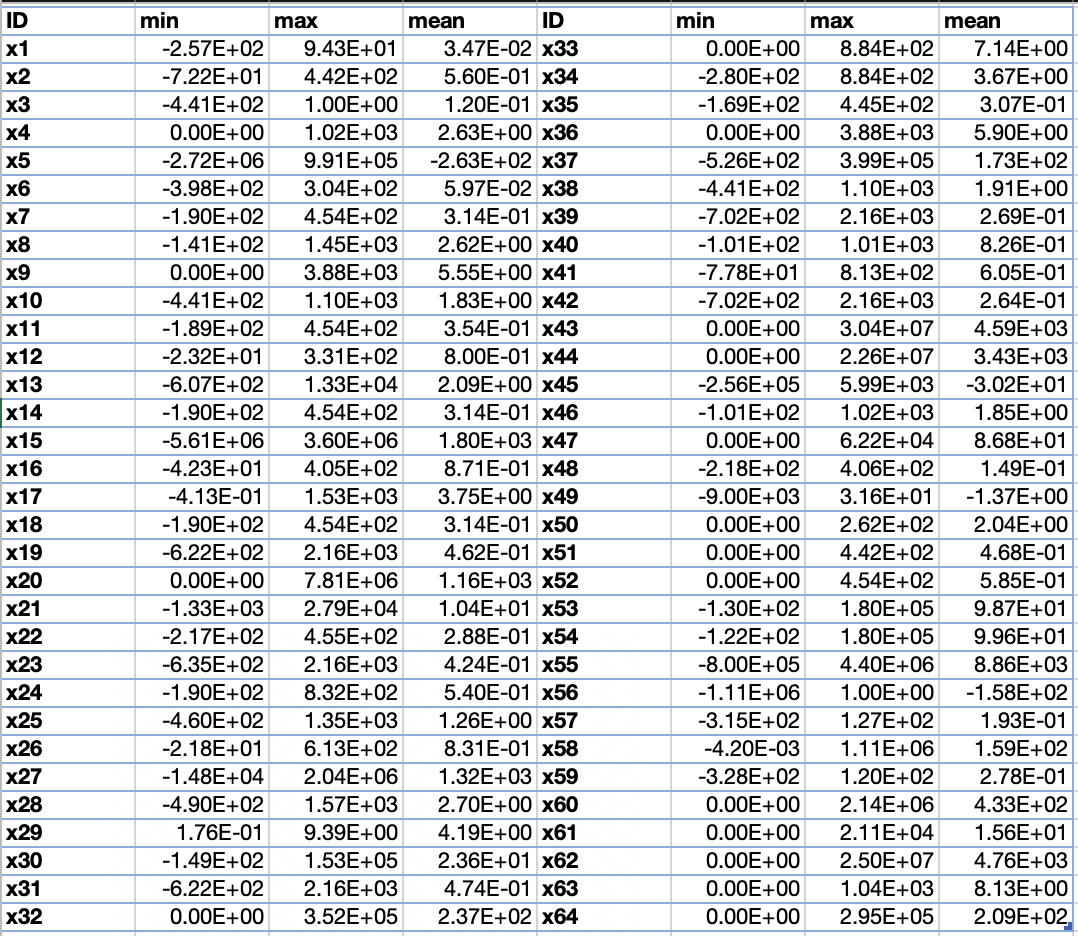
\includegraphics[width=\columnwidth]{Images/y1mmm.png}}
\caption{Min, Max and Mean for Year 1 }
\label{fig:y1mmm}
\end{figure}

% \label{sec:dataRange}
\begin{figure}[htp]
\centering
\frame{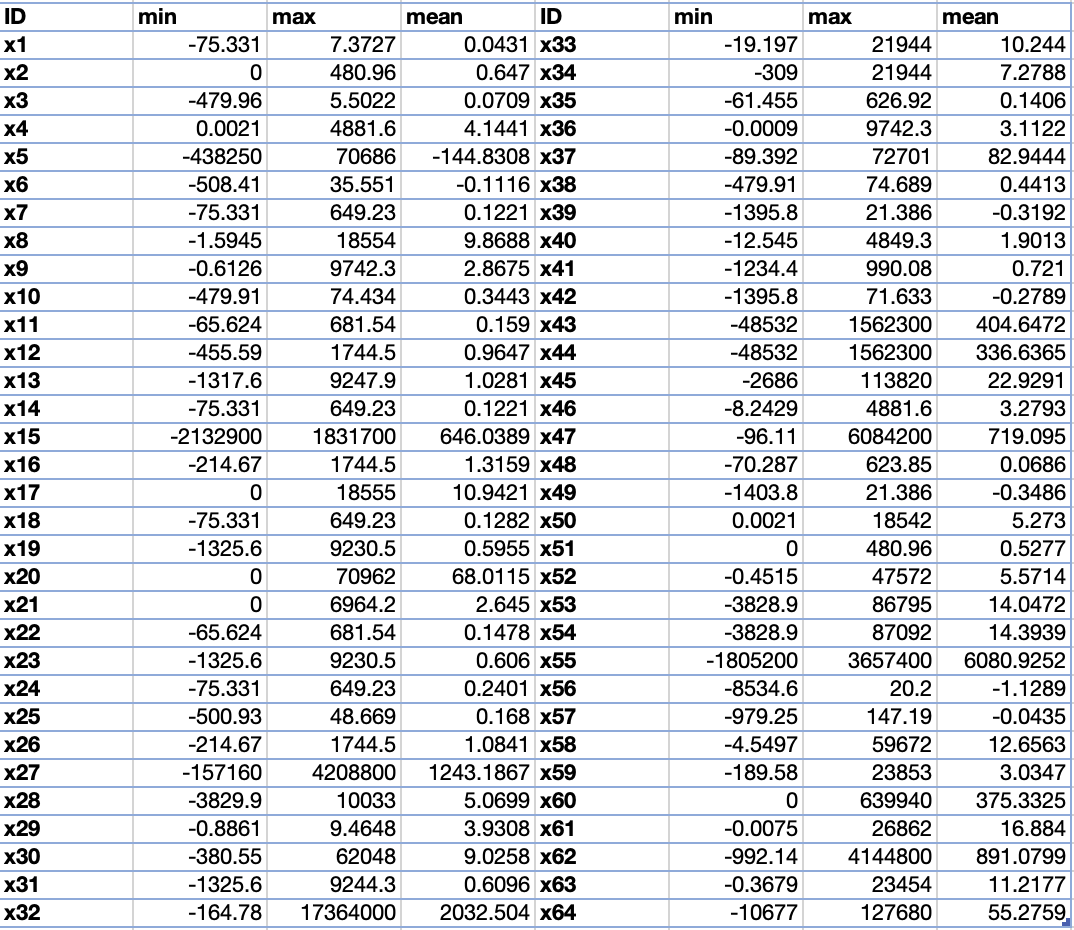
\includegraphics[width=\columnwidth]{Images/y2mmm.png}}
\caption{Min, Max and Mean for Year 2 }
\label{fig:y1mmm}
\end{figure}

% \label{sec:dataRange}
\begin{figure}[htp]
\centering
\frame{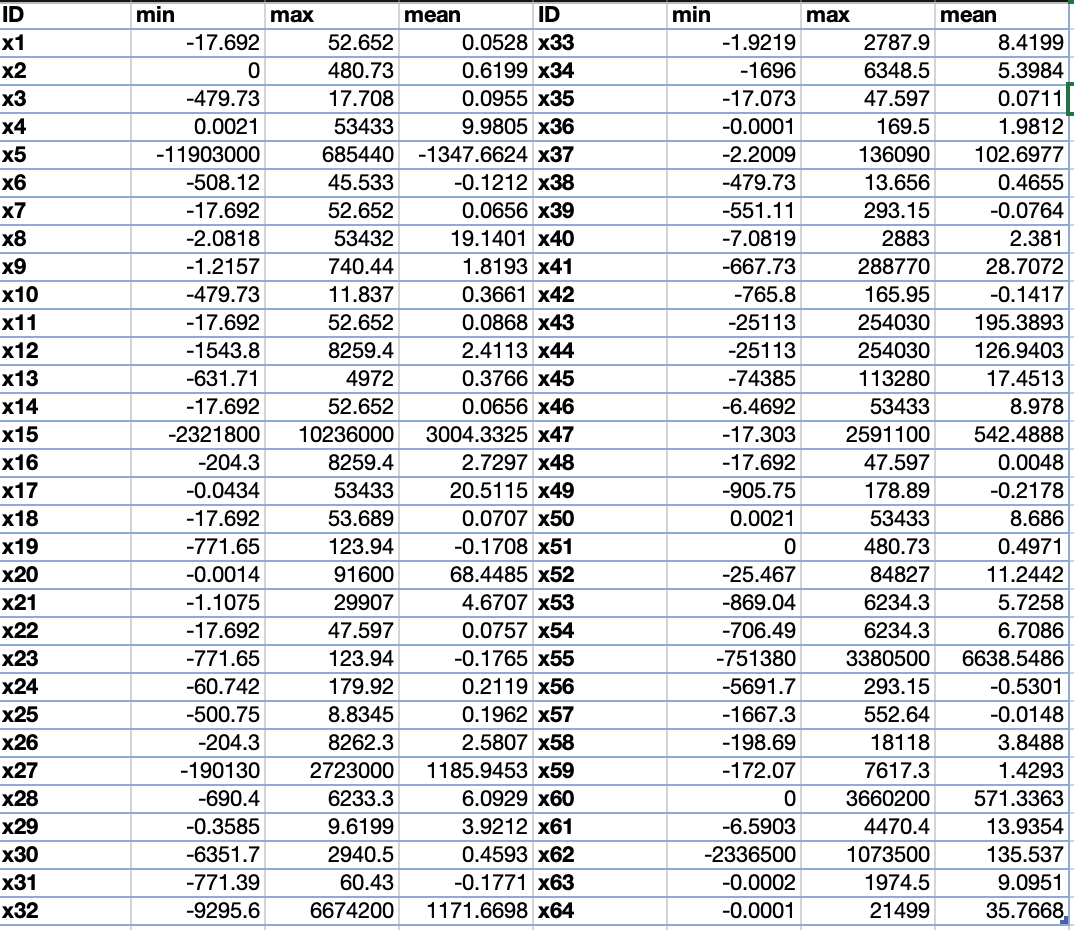
\includegraphics[width=\columnwidth]{Images/y3mmm.png}}
\caption{Min, Max and Mean for Year 3 }
\label{fig:y1mmm}
\end{figure}


\begin{figure}[htp]
\centering
\frame{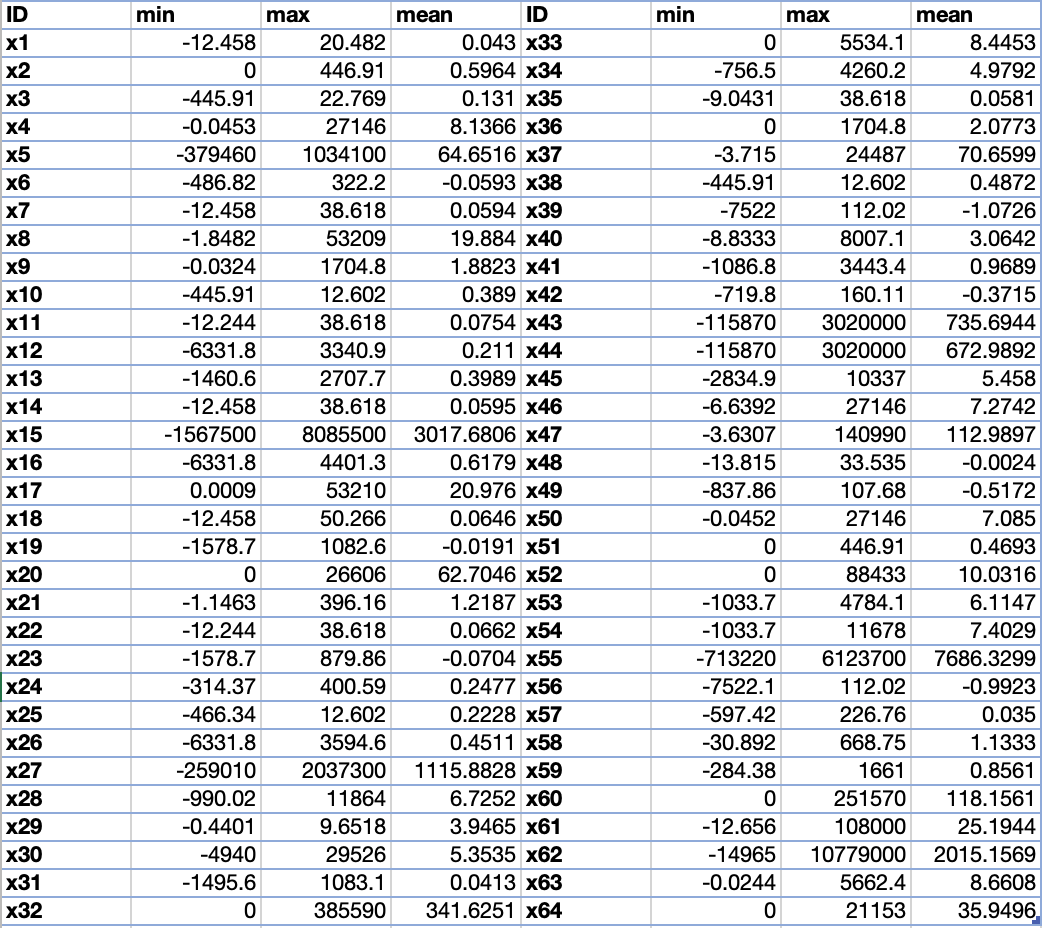
\includegraphics[width=\columnwidth]{Images/y4mmm.png}}
\caption{Min, Max and Mean for Year 4 }
\label{fig:y1mmm}
\end{figure}


\begin{figure}[htp]
\centering
\frame{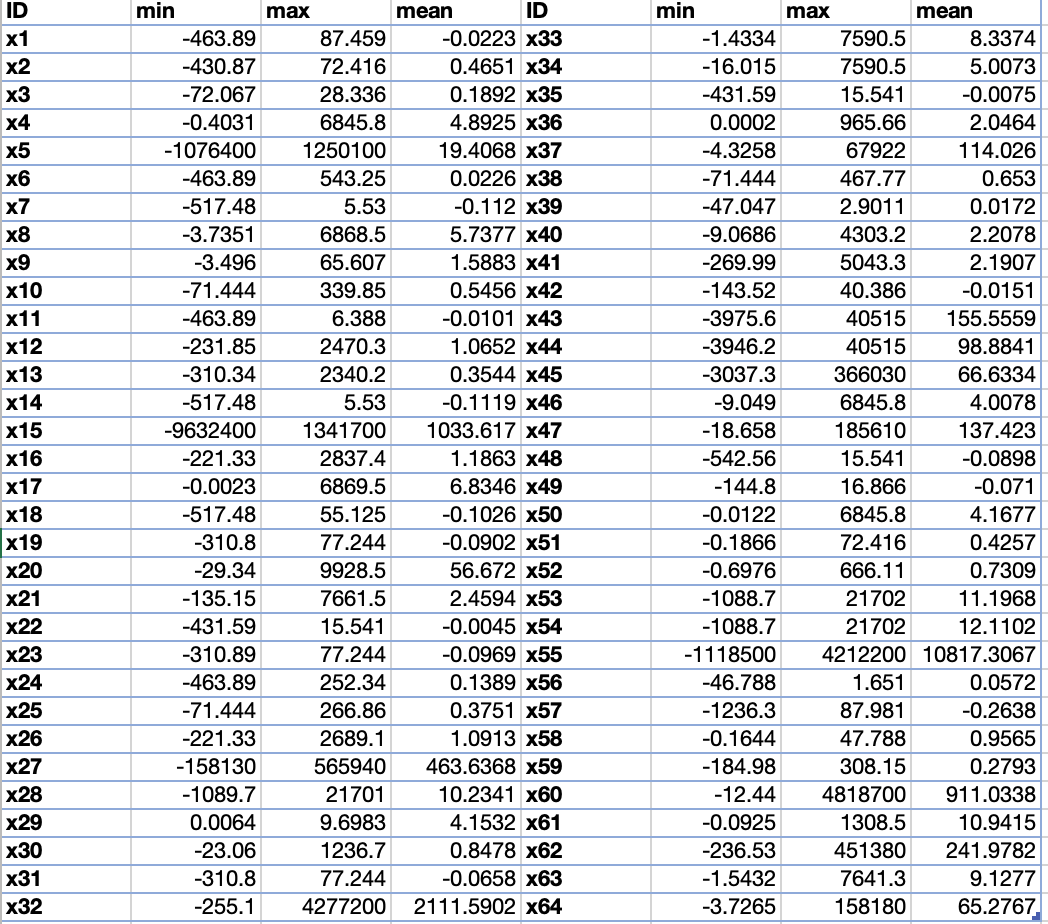
\includegraphics[width=\columnwidth]{Images/y5mmm.png}}
\caption{Min, Max and Mean for Year 5 }
\label{fig:y1mmm}
\end{figure}



\chapter{Feature Distributions}
\label{sec:corrHeat}
\begin{figure}[h]
\centering
\frame{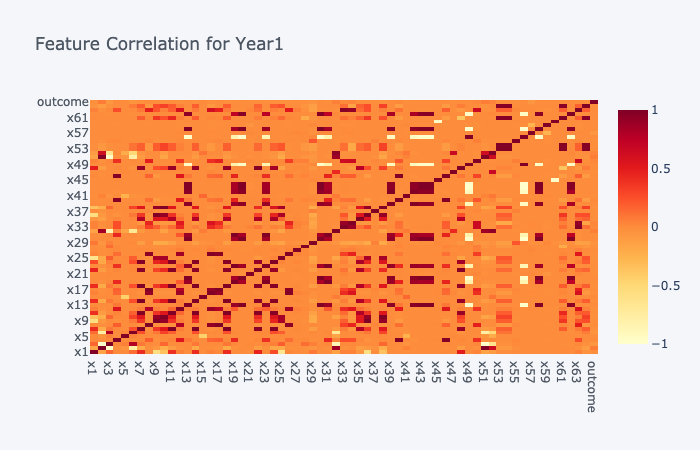
\includegraphics[width=\columnwidth]{Images/corr1.png}}
\caption{Correlation Heatmap for Year 1 }
\end{figure}

\begin{figure}
\centering
\frame{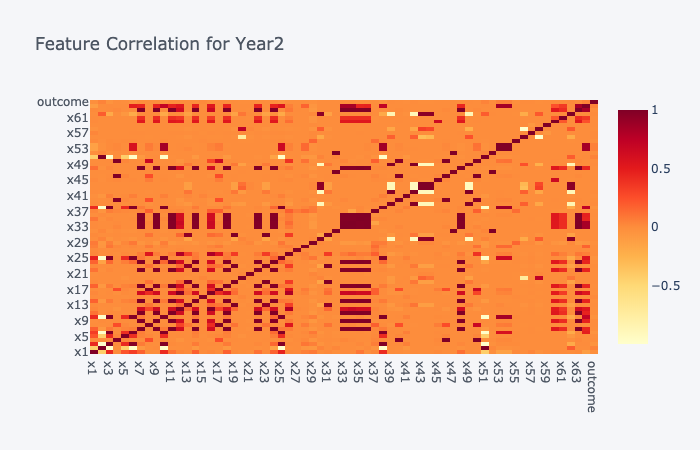
\includegraphics[width=\columnwidth]{Images/corr2.png}}
\caption{Correlation Heatmap for Year 2 }
\end{figure}

\begin{figure}
\centering
\frame{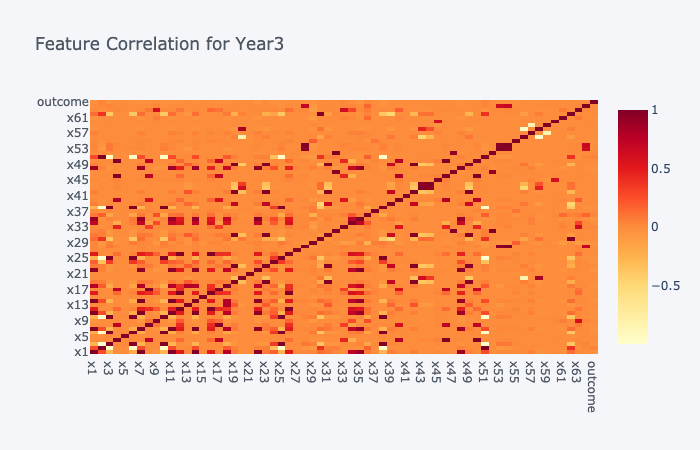
\includegraphics[width=\columnwidth]{Images/corr3.png}}
\caption{Correlation Heatmap for Year 3 }
\end{figure}

\begin{figure}
\centering
\frame{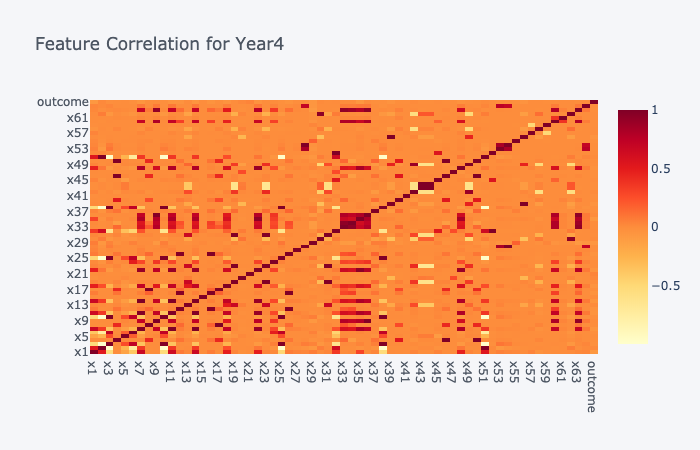
\includegraphics[width=\columnwidth]{Images/corr4.png}}
\caption{Correlation Heatmap for Year 4 }
\end{figure}

\begin{figure}
\centering
\frame{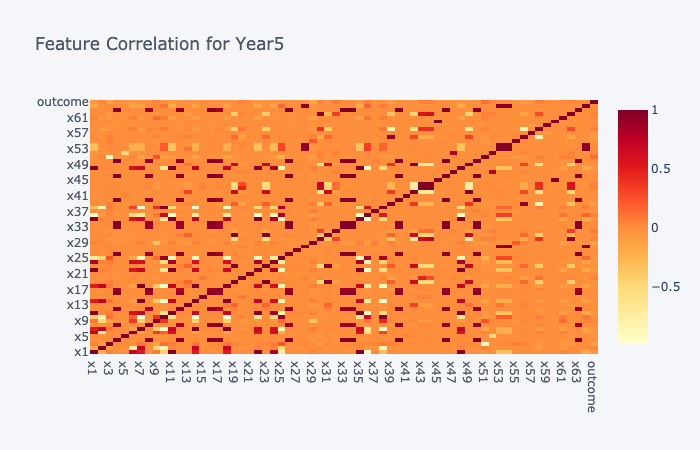
\includegraphics[width=\columnwidth]{Images/corr5.png}}
\caption{Correlation Heatmap for Year 5 }
\end{figure}

% \chapter{Logistic Regression Explained}
% \input{chapters/appendix_LR}

% \chapter{Decision Trees Explained}
% \input{chapters/appendix_DT}

% \chapter{Random Forests Explained}
% % \label{explainRF}

% Random forests are  structured through an ensemble of \textbf{d} decision trees with the following algorithm:

% \begin{enumerate}
%   \item Draw a subset of training data with random sampling by replacement (bootstrap).
%   \item Train a decision tree with the subset of training data. At each node of the tree, choose the best split of a variable from only the randomly selected m variables rather than from all the variables.
%   \item Repeat steps 1 and 2 to produce d decision trees.
%   \item Make predictions for new data by voting for the most popular class from among all of the output of the d decision trees.
% \end{enumerate}

% The Gini index (\autoref{GI}) is a popular algorithm for constructing decision trees \cite{breiman2017classification}. The Gini index is a measurement of the best split criterion based on the impurity of each node; impurity is a measure of how often a randomly chosen element from the set would be incorrectly labeled if it was randomly labeled according to the distribution of labels in the subset. The algorithm selects the optimal splitting variable and corresponding threshold value by making each node as pure as possible. Suppose $ M_n $ is the number of pieces of information reaching node n, and $ M_n^i$ is the number of data points belonging to class $ C_i$. The Gini index, $ GI_n $, of node $ n$ is thus

% \begin{equation}
% \label{GI}
%     GI_n = 1 - \sum_{i=1}^{K} (p_n^i)^2,  \hbox{where }  p_n^i = M_n^i / M_n
% \end{equation}

% A smaller Gini index value of node n represents purity, which implies that the node contains more observations from a single class. Hence, a decreasing Gini index is an important criterion for node splitting.

% \chapter{XGBoost Explained}
% % \label{explain:XGB}
% Chen and Guestrin \cite{chen2016xgboost} describe XGBboost as an ensemble of K Classification and Regression Trees (CART) \(\left\{T_{1}\left(x_{i}, y_{i}\right), \ldots . T_{K}\left(x_{i}, y_{i}\right)\right\}\) where \(x_{i}\) is the given training set of descriptors associated with a molecule to predict the class label, y, Given that a CART assigns a real score to each leaves (outcome or target), the prediction scores for individual CART is summed up to get the final score and evaluated through \(K\) additive functions, as shown in  \autoref{xgb1}:

% \begin{equation}
% \label{xgb1}
% \hat{y}_{i}=\sum_{k=1}^{K} f_{k}\left(x_{i}\right), f_{k} \in F
% \end{equation}

% where \(f_{k}\) represents an independent tree structure with leaf scores and \(F\) is the space of all CART. The regularized objective to optimize is given by  \autoref{xgb2}:

% \begin{equation}
% \label{xgb2}
% \operatorname{Obj}(\Theta)=\sum_{i}^{n} l\left(y_{i}, \hat{y}_{i}\right)+\sum_{k}^{K} \Omega\left(f_{k}\right)
% \end{equation}

% The first term is a differentiable loss function, \(l,\) which measures the difference between the predicted \(\hat{y}\) and the target \(y_{i}\). The second is a regularization term \(\Omega\) which penalizes the complexity of the model to avoid over-fiting. It is given by \(\Omega(f)= \alpha T+\frac{1}{2} \lambda \sum_{j-1}^{T} w_{j}^{2}\), where \(T\) and \(w\) are the number of leaves and the score on each leaf respectively.  $\alpha$ and $\lambda$ are constants to control the degree of regularization. Apart from the use of regularization, shrinkage and descriptor subsampling are two additional techniques used to prevent overiting \cite{sewell2008ensemble}.



% Training XGBoost is summarized as follows:

% \begin{enumerate}
%     \item For each descriptor:
%         \begin{enumerate}
%                 \item Sort the numbers
%                 \item Scan the best point to split, i.e, the lowest gain
%         \end{enumerate}
      
%     \item Choose the descriptor with the best splitting point that optimizes the training objective
%     \item Continue splitting (as in (Step 1) and (Step 2)) until the specified maximum tree depth is reached
%     \item Assign prediction score to the leaves and prune all negative nodes (nodes with negative gains) in a bottom-up order
%     \item Repeat the above steps in an additive manner until the specified number of rounds (trees K) is reached.
% \end{enumerate}


% Since additive training is used, the prediction $\hat{y}$ at step $t$ expressed as

% \begin{equation}
% \hat{y}_{i}^{(t)}=\sum_{k=1}^{K} f_{k}\left(x_{i}\right)=\hat{y}_{i}^{(t-1)}+f_{t}\left(x_{i}\right)
% \end{equation}

% And the objective function can be written as:

% \begin{equation}
% \operatorname{Obj}(\Theta)^{(t)}=\sum_{i}^{n} l\left(y_{i}, \hat{y}_{i}^{(t-1)}+f_{t}\left(x_{i}\right)\right)+\Omega\left(f_{t}\right)
% \end{equation}

% % After taking a Taylor expansion where \(g_{i}=\partial_{\hat{y}_{i}^{(t-1)}} l\left(y_{i}, \hat{y}_{i}^{(t-1)}\right)\) and \(h_{i}=\partial^{2}_{\hat{y}_{i}^{(t-1)}} l\left(y_{i}, \hat{y}_{i}^{(t-1)}\right)\) are respectively first and second order statistics on the loss function, a simplified objective function without constants at step \(t\) is as follows: 

% % \begin{equation}
% % \operatorname{Obj}(\Theta)^{(t)}=\sum_{i=1}^{n}\left[g_{i} f_{t}\left(x_{i}\right)+\frac{1}{2} h_{i} f_{t}^{2}\left(x_{i}\right)\right]+\Omega\left(f_{t}\right)
% % \end{equation}



% % The objective function can be written by expanding the regularization term as
% % \begin{equation}
% % \begin{aligned}
% % \operatorname{Obj}(\Theta)^{(t)} &=\sum_{i=1}^{n}\left[g_{i} f_{t}\left(x_{i}\right)+\frac{1}{2} h_{i} f_{t}^{2}\left(x_{i}\right)\right]+\gamma T+\frac{1}{2} \lambda \sum_{j=1}^{T} w_{j}^{2} \\
% % &=\sum_{j=1}^{T}\left[\left(\sum_{i \in I_{j}} g_{i}\right) w_{j}+\frac{1}{2}\left(\sum_{i \in I_{j}} h_{i}+\lambda\right) w_{j}^{2}\right]+v T
% % \end{aligned}
% % \end{equation}

% % where \(I_{j}=\left\{i | q\left(x_{i}\right)=j\right\}\) is the instance set of leaf \(j\), for a given structure \(q(x)\) the optimal leaf weight, \(w_{j}^{*},\) and the optimal objective function which measure how good the structure is are given by \autoref{xgb7}.

% % \begin{equation}
% % \label{xgb7}
% % \begin{array}{c}
% % w_{j}^{*} = -\frac{G_{j}}{H_{j}+\lambda} \\
% % O b j^{*} = -\frac{1}{2} \sum_{j=1}^{T} \frac{G_{j}^{2}}{H_{j}+\lambda}+\mathrm{yT}
% % \end{array}
% % \end{equation}

% % % where $\(G_{j}=\sum_{i \in I_{j}} g_{i}$ and $\(H_{j}=\sum_{i \in I_{j}} h_{i}\) \\ \\
% % $$
% % \begin{array}
% % \text \hbox{ where } G_{j}=\sum_{i \in I_{j}} g_{i} G_{j}=\sum_{i \in I_{j}} g_{i} \text { and } H_{j}=\sum_{i \in I_{j}} h_{i}
% % \end{array}
% % $$

% % \autoref{xgb10} is used to score a leaf node during spliting. The first, second and third term of the equation stands for the score on the left, right and the original leaf respectively. Moreover, the final term, \(\mathrm{y}\), is regularization on the additional leaf.

% % \begin{equation}
% % \label{xgb10}
% % \text {Gain}=\frac{1}{2}\left[\frac{G_{L}^{2}}{H_{L}+\lambda}+\frac{G_{R}^{2}}{H_{R}+\lambda}-\frac{\left(G_{L}+G_{R}\right)^{2}}{H_{L}+H_{R}+\lambda}\right]-\mathrm{y}
% % \end{equation}


\chapter{Python Libraries used for Project}
\begin{table}[h!]
\begin{center}
 \begin{tabular}{ | p{7.7cm}| p{7cm} | }
 \hline
  Library & Description

  \\ [0.5ex] 
 \hline\hline
     numpy & Data organization and statistical operations. \\
    \hline pandas & Data manipulation and analysis. Storing and manipulating numerical tables. \\
    \hline matplotlib, plotly and seaborn & Plotting libraries \\
    % \hline plot & Plotting library \\
    \hline missingno & Generate nullity matrices and correlation heatmaps for missing data. \\
    \hline fancyimpute & Perform k-NN and MICE imputation \\
    \hline impyute & Perform EM imputation \\
    \hline sklearn.model\_selection.StratifiedKFold & Perform Stratified K-Fold Cross Validation \\
    \hline imblearn.over\_sampling.SMOTE & Perform SMOTE Oversampling \\
    \hline sklearn.linear\_model.LogisticRegression & Logistic Regression Classifier \\
    \hline sklearn.tree.DecisionTreeClassifier & Decision Tree Classifier \\
    \hline sklearn.ensemble.RandomForestClassifier & Random Forest Classifier \\
    \hline imblearn.ensemble.BalancedBaggingClassifer & Balanced Bagging Classifier \\
    \hline xgboost.XGBClassifier & Extreme Gradient Boosting classifier \\
    \hline sklearn.metrics & Performance evaluation metrics like accuracy score, recall, precision, ROC curve, etc. \\
\hline

\end{tabular}
\end{center}

	\caption{Libraries used for the project.}
\label{table:LibUsed}
\end{table}


% \begin{tabular}{|l|l|}
% \hline \multicolumn{1}{|c|} { Library } & \multicolumn{1}{|c|} { Description } \\
% \hline numpy & Data organization and statistical operations. \\
% \hline pandas & Data manipulation and analysis. Storing and manipulating numerical tables. \\
% \hline matplotlib & Plotting library \\
% \hline scipy.io & Loading arff raw data \\
% \hline missingno & Generate nullity matrices and correlation heatmaps for missing data. \\
% \hline fancyimpute & Perform k-NN and MICE imputation \\
% \hline impyute & Perform EM imputation \\
% \hline sklearn.preprocessing.Imputer & Perform Mean imputation \\
% \hline sklearn.model_selection.KFold & Perform K-Fold Cross Validation \\
% \hline imblearn.over_sampling.SMOTE & Perform SMOTE Oversampling \\
% \hline xgboost.XGBClassifier & Extreme Gradient Boosting classifier \\
% \hline sklearn.ensemble.RandomForestClassifier & Random Forest Classifier \\
% \hline sklearn.linear_model.LogisticRegression & Logistic Regression Classifier \\
% \hline imblearn.ensemble.BalancedBaggingClassifie r & Balanced Bagging Classifier \\
% \hline sklearn.tree.DecisionTreeClassifier & Decision Tree Classifier \\
% \hline sklearn.naive_bayes.GaussianNB & Gaussian Naive Bayes Classifier \\
% \hline sklearn.metrics & Performance evaluation metrics like accuracy score, recall, precision, ROC curve, etc. \\
% \hline
% \end{tabular}

\end{appendices}


\bibliographystyle{plain}
\bibliography{mybibfile}

\end{document}
